%====================================================================

\documentclass[10pt, conference, compsocconf]{IEEEtran}

%====================================================================

% !TEX root = ../main.tex

% = = = Compact Bibliography
%\usepackage{bibspacing}
%\setlength{\bibspacing}{\baselineskip}

%------------------------IEEE----------------------%

% = = = IEEE Recommended
\usepackage{mdwmath}
\usepackage{mdwtab}
\usepackage{eqparbox}

% = = = IEEE Recommended (Double-column)
%\usepackage{fixltx2e}
\usepackage{stfloats}

% NOTE: IEEE does not allow algorithm2e

%------------------------Packages----------------------%

% = = = Graphics
\usepackage[pdftex]{graphicx}
\graphicspath{{figures/}}
\DeclareGraphicsExtensions{.jpg,.png}

% = = = Subfig (note not subfigure)
\usepackage[caption=false,font=footnotesize]{subfig}

% = = = Math Symbols
\usepackage{amsmath}
%\usepackage{amstext,amssymb,amsthm}
\usepackage{bbm}
\usepackage{stmaryrd}

% = = = Other
\usepackage{array}
\usepackage{color}
\usepackage[hyphens]{url}
\usepackage[pdftitle=Title,pdfauthor=Anonymous]{hyperref}

%------------------------END----------------------%  
  


% !TEX root = ../main.tex

%------------------------Custom Commands----------------------%

% = = = Latin Short-forms (ie, eg, etc, et al)
\usepackage{xspace}
\newcommand{\etal}{\textit{et al.}\xspace}
\newcommand{\etc}{\textit{etc.}\xspace}
\newcommand{\ie}{\textit{i.e.,}\xspace}
\newcommand{\eg}{\textit{e.g.,}\xspace}
\newcommand{\cf}{\textit{cf.}\xspace}
\newcommand{\supra}{\textit{Supra}\xspace}

% = = = Arrow -> (\lt)
\newcommand{\lt}{$\rightarrow$\xspace}

% = = = Keywords (kw)
\newcommand{\kw}[1]{\textsf{#1}}

% = = = Colored text (textblue)
\newcommand{\textblue}[1]{\textcolor{blue}{#1}}

% = = = Compact Lists (compactlist, compactlistn)
\newenvironment{compactlist}
  {\begin{itemize} 
  \setlength{\itemsep}{0pt} 
  \setlength{\parskip}{0pt}} 
  {\end{itemize}}
  
\newenvironment{compactlistn}
  {\begin{enumerate} 
  \setlength{\itemsep}{0pt} 
  \setlength{\parskip}{0pt}} 
  {\end{enumerate}}
  
\renewcommand{\labelitemi}{$\bullet$}
  

%------------------------Crypto----------------------%  

% = = = Zp, Gq and Zq
\newcommand{\Zp}{\mathbb{Z}^{*}_{p}}
\newcommand{\Zq}{\mathbb{Z}_{q}}
\newcommand{\Gq}{\mathbb{G}_{q}}

% = = = Encryption, etc.
\newcommand{\Enc}[1]{\mathsf{Enc}(#1)}
\newcommand{\EncB}[1]{\llbracket #1 \rrbracket}
\newcommand{\ReRand}[1]{\mathsf{ReRand}(#1)}
\newcommand{\Hash}[1]{\mathcal{H}(#1)}
\newcommand{\Sign}[1]{\mathsf{Sig}(#1)}
\newcommand{\Comm}[1]{\mathsf{Comm}(#1)}
\newcommand{\Open}[1]{\mathsf{Open}(#1)}

% = = = Tuples
\newcommand{\tuple}[1]{\left \langle #1 \right \rangle}


%-------------------Custom for Paper----------------------%

% = = = Name
\newcommand{\Name}{\textsf{System Name}\xspace}


%-----------------------Notes------------------------------------%
\usepackage{todonotes}
\newcommand{\anote}[1]{\todo[inline]{Arkady:  #1}}
\newcommand{\bnote}[1]{\todo[inline]{Ben:  #1}}
\newcommand{\rnote}[1]{\todo[inline]{Rob: #1}}


\usepackage{draftwatermark}
\SetWatermarkColor[gray]{0.9}

%====================================================================

\IEEEoverridecommandlockouts

\begin{document}
\title{SoK: Blockchain Technology and Its Potential Use Cases}
%TODO: This needs to be anonymized when submitted.

\makeatletter
\newcommand{\linebreakand}{%
	\end{@IEEEauthorhalign}
	\hfill\mbox{}\par
	\mbox{}\hfill\begin{@IEEEauthorhalign}
}
\makeatother

\makeatletter
\def\blfootnote{\gdef\@thefnmark{}\@footnotetext}
\makeatother

\author{
%	Anonymous
	\IEEEauthorblockN{Scott Ruoti}
	\IEEEauthorblockA{
		University of Tennessee, Knoxville\\
		MIT Lincoln Laboratory\IEEEauthorrefmark{1}\\
		ruoti@utk.edu
	}

	\and
	
	\IEEEauthorblockN{Ben Kaiser}
	\IEEEauthorblockA{
		Princeton University\\
		MIT Lincoln Laboratory\IEEEauthorrefmark{1}\\
		bkaiser@princeton.edu
	}

	\and
	
	\IEEEauthorblockN{Arkady Yerukhimovich}
	\IEEEauthorblockA{
		George Washington University\\
		MIT Lincoln Laboratory\IEEEauthorrefmark{1}\\
		arkady@gwu.edu
	}

	\linebreakand

	\IEEEauthorblockN{Jeremy Clark}
	\IEEEauthorblockA{
		Concordia University\\
		j.clark@concordia.ca
	}

	\and

	\IEEEauthorblockN{Robert Cunningham}
	\IEEEauthorblockA{
		Carnegie Mellon University\\
		Software Engineering Institute\\
		MIT Lincoln Laboratory\IEEEauthorrefmark{1}\\
		robertkcunningham@cmu.edu
	}	
}

\maketitle

\blfootnote{\IEEEauthorrefmark{1}The majority of this work was completed while these authors worked at MIT Lincoln Laboratory.}

%====================================================================

% !TEX root = ../main.tex

\begin{abstract}
Bitcoin's success has led to significant interest in its underlying components, particularly Blockchain technology.
Over 10 years after Bitcoin's initial release, the community still suffers from 
a lack of clarity regarding what properties defines Blockchain technology, its 
relationship to similar technologies, and which of its proposed use-cases are 
tenable and which are little more than hype.
In this paper we answer four common questions regarding Blockchain technology: (1) what exactly is Blockchain technology, (2) what capabilities does it provide, and (3) what are good applications for Blockchain technology, and (4) how does it relate to other approache distributed technologies (e.g., distributed databases).
We accomplish this goal by using grounded theory---a structured approach to gathering and analyzing qualitative data---to thoroughly analyze a large corpus of literature on Blockchain technology.
This method enables us to answer the above questions while limiting researcher bias, separating thought leadership from peddled hype and identifying  open research questions related to Blockchain technology.
%We also discuss lessons learned from our analysis of this space using this approach.
The audience for this paper is broad as it aims to help researchers in a 
variety of areas come to a better understanding of Blockchain technology and 
identify whether it may be of use in their own research.
\end{abstract}

\begin{IEEEkeywords}
Blockchain, decentralized governance, distributed ledger, provenance, auditability, resilience.
\end{IEEEkeywords}
\IEEEpeerreviewmaketitle
\thispagestyle{plain}
\pagestyle{plain}

%====================================================================

% !TEX root = ../main.tex

\section{Introduction}
%\rnote{I think that we need to start with the notion of an authenticated data structure or hash chain used to establish the integrity of data, given the title of the paper.  What is the right reference?}

In 1982, David Chaum~\cite{Cha82} proposed using blind signatures to allow for untraceable payments.
Later, Chaum et al.~\cite{chaum1988untraceable} expanded this idea into a fully fleshed out system, eCash.
eCash was the first cryptocurrency---i.e., ``a digital currency in which encryption techniques are used to regulate the generation of units of currency and verify the transfer of funds operating independently of a [nation-state-controlled] central bank.''\footnote{\url{https://en.oxforddictionaries.com/definition/cryptocurrency}}
However, early cryptocurrencies still required the presence of a central party to help manage the creation and transfer of funds.

Two decades after eCash was first proposed, an author using the pseudonym Satoshi Nakamoto wrote a white paper describing Bitcoin, a new decentralized cryptocurrency~\cite{Nak08}.
Unlike centralized cryptocurrencies which rely on a set of known entities to operate, Bitcoin uses a proof-of-work-based scheme~\cite{DN93,back1997partial} to allow the general public to maintain the system.
To incentivize public participation, Bitcoin pays participants (known as miners) for solving the proof-of-work puzzles.
While Bitcoin's building blocks were not novel, the composition of these properties into a single system was a meaningful contribution~\cite{Narayanan17} which led the cryptocurrency to become the first to achieve widespread popularity and usage.

At the peak of its popularity, Bitcoin's market capitalization reached \$835.69 billion (USD), though at the time of this writing it has seen a decrease in both its stature and market capitalization (\$67.21 billion).
Nevertheless, there remains significant interest in the question of whether the technology underlying Bitcoin---known as \emph{Blockchain technology} or {Blockchain} for short---could be used to build other interesting cryptocurrencies or distributed systems.
In particular, we have consistently heard researchers, businesses, and governments ask the following three questions related to Blockchain technology: (1) what exactly is Blockchain technology, (2) what capabilities does it provide, and (3) what are good applications for Blockchain technology.%, and (4) how does it relate to other approache distributed technologies (e.g., distributed databases).

To answer these questions, it is insufficient to consider academic sources alone.
While there have been several academic overviews written in this space, they have not addressed these general question regarding Blockchain technology, but rather surveyed particular systems or technical properties: Bitcoin~\cite{BMC+15,Narayanan17}, payment privacy~\cite{Conti17}, security and performance~\cite{Gervais16}, scalability~\cite{Croman16}, and consensus protocols~\cite{Bano17,garay2018consensus}.
In contrast, there has been significant work from non-academic sources (hereafter referred to as \emph{industry}) attempting to answers the questions as they search for applications and new product offerings that could be enabled by Blockchain technology.
Unfortunately, much of this work is fueled by hype and lacks the peer-review process and rigor expected of academic literature.

To address these limitations in our analysis of literature produced by industry we applied a grounded theory methodology~\cite{glaser1965constant,strauss1990basics,corbin1990grounded} (also known as the constant comparative method).
This allowed us to extract valuable technical insights out from the hype and technical misunderstandings that permeate this body of work.
Based on this analysis of data from industry, interspersed with our own knowledge and a review of the academic literature, we are able to answer the three questions commonly asked in relation to Blockchain technology.

While many of the results in this work might not be surprising to some readers, our experience suggests that knowledge of Blockchain technology is neither universal nor complete within the security community.
Taken together, the results in this paper represent the most complete overview of Blockchain technology and its potential use cases available in a single work and are intended to serve as an aid for researchers as they field questions related to Blockchain and as they explore whether Blockchain technology is relevant to their personal research areas. More concretely, our key contributions are:

\begin{enumerate}
	\item \textbf{Defining the key technical properties of Blockchain technology.}
	Based on the results of our analysis, we identify three key properties for Blockchain technology: shared governance and operation, the use of an append-only ledger, and replication of data.
	Blockchain systems are governed and operated by a distributed and decentralized collective of entities that ensure that all operations are valid.
	These operations are recorded in an append-only ledger that provides full-system provenance.
	This ledger is also replicated by a set of governing parties, providing resilience against data loss and malicious modification of data.
	We also discuss associated technical properties that Blockchain makes use of.
	
	\item \textbf{Identifying the capabilities provided by Blockchain technology.}
	Our results demonstrate that Blockchain provides several important capabilities for use in building  systems.
	First, Blockchain systems inherently track their full-system provenance, and this provenance data allows for the system to be audited by miners and potentially by outside parties.
	This provenance data is also useful in tracking assets monitored or managed by the Blockchain system (e.g., supply chain management, cryptocurrencies).
	Second, Blockchain technology provides access control for the assets it monitors or manages and can allow operations on these assets to be pseudonymous.
	Third, the provenance information and replication of that information among all miners provides significant resilience against accidental data loss or malicious modification of the data.
	Fourth, Blockchain systems can embed executable programs that can automatically execute as appropriate and enjoy the benefits of Blockchain technology's other capabilities.
	
	\item \textbf{Identifying groups of applications (i.e., use cases) that are most likely to benefit from Blockchain technology.}
	Within the literature we analyzed there was a range of potential applications for Blockchain technology.
	We group these applications into a set of use cases and then discuss the likelihood that individual applications within the use case would benefit from the use of Blockchain technology.
	Example use cases include cryptocurrencies, asset management, and multi-organization data sharing.
	
	%TODO: These need to be updated when I work through these sections and the discussion.
	\item \textbf{Detailing challenges and limitations related to Blockchain technology.}
	As part of our review of the literature, we identified several important challenges and limitations for Blockchain technology: scalability, smart contract correctness and dispute resolution, stapling of on-chain tokens to off-chain assets, key management, and regulation.
	Many of this challenges represent important research questions with interesting potential for future research.
%	In this paper, we also survey the academic research that has already been conducted in regards to Blockchain technology.

%	\item \textbf{Describe how Blockchain technology fits in relation to other distributed databases.}
%	We provide a taxonomy and flow chart that describes how Blockchain technology relates to other distributed databases.
%	This taxonomy demonstrates that Blockchain technology is the most complex of the related distributed databases.
%	As such, we recommend that applications leverage Blockchain technology only if they need the shared governance, provenance, auditability and resilience provided by Blockchain technology.

	
\end{enumerate}

% !TEX root = ../main.tex

\section{Methodology}
\label{sec:method}

In addition to a survey of academic literature, we conducted a rigorous textual analysis of non-academic sources (hereafter referred to as industry),
%\footnote{Here, we consider industry broadly: corporations, small and medium business, startups, and consortia.}
including but not limited to sources from the technology, financial, and healthcare sectors.
This analysis provides the basis for the results discussed in this paper.
While there is valuable information to be learned from industry, analyzing 
these sources brings challenges: (a) a lack of precise terminology and 
discussion, (b) inclusion of hype, and (c) researcher bias.

%\begin{enumerate}
%	\item \emph{Lack of precise terminology and discussion.}
%	In our review of materials from industry, we found that the same concepts were often described using divergent and imprecise terminology, leading to white papers that are difficult to understand and provide muddled descriptions of capabilities and use cases.
%	Additionally, while there is a fair bit of factually inaccurate information in materials from industry (e.g., several documents claimed cryptographic signatures provide confidentiality), in several cases we  observed an accurate description of an idea that was phrased in such a way as to make it seem incorrect under cursory examination. Some of those ideas were assembled in ways that are interesting to academics, if one takes the time to work through the material.
%	In this regard, materials from industry represent a trove of useful information obscured by imprecise terminology and discussion.
%	
%	\item \emph{Inclusion of hype.}
%	Much of the material from industry includes visionary statements (i.e., hype) about how Blockchain technology will change business practices, power dynamics and the way the world works.
%	This hype is a mixture of realistic use cases that can benefit from Blockchain technology (e.g., anonymous payments~\cite{chaum1988untraceable}) and ideals that far transcend any technical solution (e.g., removing the need for governments).
%	Unfortunately, unlike what one would expect in academic literature, the materials from industry often intermingle hype with technical details. This at least partially explains why some in academia are quick to dismiss sources from industry.
%	
%	\item \emph{Researcher bias.}	
%	Researcher bias is an obvious problem in any literature review---regardless of whether the source is academia or industry---and one that is often not explicitly addressed in systemization papers.
%	The potential for bias is even stronger when reviewing materials from industry because the two issues described above (lack of precise terminology and hype) make it easy for researchers to dismiss out of hand ideas proposed by industry.
%%	Additionally, being aware of the academic pedigree of Blockchain technology can make it easy to overlook the interesting use cases enabled by the composition of existing primitives.
%	
%\end{enumerate}

To address these limitations, we employed a well-established research 
method---\emph{grounded 
theory}~\cite{corbin1990grounded,wolfswinkel2013using}---to rigorously analyze 
the data in a way that directly addresses each of the above issues.
%~\cite{glaser1965constant,strauss1990basics,corbin1990grounded}
%Grounded theory is used to analyze qualitative data sources (e.g., user stories, interviews) and extract the underlying data and processes described across the myriad of gathered sources.
%\footnote{Grounded theory identifies data and processes that are supported across the body of sources and is not a method for creating a fine-grained breakdown of an individual document.}
Grounded theory is designed to help researchers identify data and processes 
within qualitative data sources generated by humans and filled with imprecise 
terminology and descriptions.
Additionally, grounded theory limits the impact of researcher bias, ensuring that the data and processes are derived from the data and not from the researchers' preconceived notions of what the data says.
Our hope was that it would also help separate hype from the underlying facts, 
and based on the clarity of our results we believe it did so.
%As readers may be unaware of the grounded theory methodology, in this section we describe the methodology in more depth.

%In the remainder of this section, we describe the data we gathered as well as the grounded theory process used to evaluate it.

%The idea of using grounded theory for literature review is not new
%%~\cite{wolfswinkel2013using,yang2012descriptive}
%and this method has been used in thousands of studies examining qualitative data.
%%\footnote{As evidence of its wide use, the top-cited paper describing grounded theory has 62,951 citations as of writing.}
%%TODO: This needs to be deanonymized when published.
%For these reasons---and based on our own experience with the method~\cite{ruoti2017weighing}---we were confident this method would allow us to successfully accomplish our research goals.

%In the remainder of this section we first describe how we gathered industry materials for our grounded theory analysis.
%Next, we describe the grounded theory process in some detail, as it may be unfamiliar to readers in this field.
%Lastly, we describe an academic literature review we conducted to enhance the results of our grounded theory analysis.

\subsection{Industry Material Gathering}
%Beginning in the summer of 2016
%We gathered documents published regarding Blockchain technology, including both materials from industry and academia, though this section will focus on only the former.
We gathered materials using a variety of methods:

\begin{itemize}
	\item Following RSS feeds that track news and publications related to 
	Blockchain technology.% (e.g., 
	%CoinDesk).%\footnote{\url{https://coindesk.com}}).
	\item Downloading materials published by Blockchain consortiums (e.g., 
	Hyperledger, Decentralized Identity Framework).% and their members (e.g., 
	%IBM, Microsoft, Gem).
%	\item Downloaded materials published by Blockchain consortiums (e.g., Hyperledger\footnote{\url{https://www.hyperledger.org/}}, Decentralized Identity Framework\footnote{\url{http://identity.foundation/}}) and their members (e.g., IBM, Microsoft, Gem).
	\item Reviewing documents from major accounting firms, banks, and tech companies.
	\item Browsing news articles and blog posts related to Blockchain technology.% This included articles which gave lists of interesting Blockchain papers.
	\item Reviewing submissions to the ONC Blockchain in Health Care Competition.
	%\footnote{\url{https://www.healthit.gov/topic/grants-contracts/announcing-blockchain-challenge}}.
\end{itemize}

When reviewing these materials, we would also follow references and include those documents if we believed they were relevant.
In total, we collected 132 documents which can be split into three categories: high-level overviews, system white papers, and Blockchain commentaries.

%\begin{itemize}
%	\item \emph{High-Level Overviews.} These were often prepared by investment firms and gave high level overviews of Blockchain technology. They would also reference various efforts at using Blockchain in practice.
%	\item \emph{System White Papers.} These papers would describe how Blockchain technology was used in a specific system, or more frequently a system proposal.
%	\item \emph{Blockchain Commentaries.} These were generally shorter documents that would discuss a specific facet of Blockchain technology in greater depth than we saw in other documents.
%\end{itemize}

\subsection{Grounded Theory Data Analysis}
Four members of our group participated in the analysis of collected documents.
We continued gathering and reviewing documents until each of us felt that the last 3--5 documents we had read revealed no new information regarding Blockchain technology; this is a commonly accepted stopping criteria in grounded theory that ensures that all core (i.e., not one-off) ideas have been identified.
Throughout this analysis we kept detailed research notes that outlined our thoughts as we reviewed and analyzed the literature.
Additionally, we conducted intensive discussion between the various researchers to ensure that we were correctly understanding and evaluating the source material.
%As is often the case in grounded theory, these notes and discussion were every bit as important, if not more so, than the concepts, categories, and theories we generated.

Our analysis ultimately revealed a set of 68 interconnected concepts that 
define Blockchain technology.
These concepts are grouped into five categories:

\begin{itemize}
	\item \emph{Technical properties (Figure~\ref{fig:technical-properties}).}
	%,~\ref{fig:technical-properties-full}).}
	Technical properties are the components that make up Blockchain technology. 
	Examples include decentralized governance, a consensus protocol, and an 
	append-only transaction ledger.
	
	\item \emph{Capabilities (Figure~\ref{fig:Capabilities}).}
	Capabilities are the high-level features provided by the technical 
	properties. Examples include automatic executions (i.e., smart contracts), 
	internal auditability, and access control.
	
	\item \emph{Technical primitives.}
	Primitives are the building blocks used to construct the technical properties and capabilities of Blockchain technology. Examples include timestamps, hashchains, and peer-to-to-peer communication.
	
	\item \emph{Use cases.}
	Use cases are classes of systems that the literature identified as 
	applications of Blockchain technology. Examples include crytocurrencies, 
	supply chain management, and identity management.
	
	\item \emph{Normative properties.} 
	%(Figure~\ref{fig:normative-properties})
	Normative properties represent what people hope to achieve using Blockchain technology. 
	Importantly, these properties are not provided by the use of Blockchain 
	technology as are the technical properties and capabilities. Rathey they 
	typically require the careful design of larger systems of which Blockchain 
	technology may only be a small component.
	In general, normative properties strongly relate to the hype surrounding Blockchain technology
	%.
	and as such we do not discuss them further in this article.
	%		Examples include public participation, trustlessness, and censorship resistance.
\end{itemize}

%\subsection{Grounded Theory Data Analysis}
%After collecting our initial set of 104 documents, we analyzed them using grounded theory.
%This methodology splits analysis of the documents into four stages: open coding, axial coding, selective coding, and theory generation.
%Throughout the analysis of the documents we kept detailed research notes that outlined our thoughts as we reviewed and analyzed the literature.
%Additionally, we conducted intensive discussion between the various researchers to ensure that we were correctly understanding and evaluating the source material.
%As is often the case in grounded theory, these notes and discussion were every bit as important, if not more so, than the concepts, categories, and theories we generated.
%
%\subsubsection{Stage 1---Open Coding}
%In this first stage, documents were assigned to one of four reviewers who would read the document and assign codes to words and sentences in the document.
%These codes were generated using a mixture of open coding (assigning a code that summarizes the document's statement) and in situ coding (using the document's own words as the code).
%To ensure that we were assigning the correct codes, we paid careful attention to the context of each statement.
%
%In particular, reviewers made sure to code the following four concepts found in documents:
%\begin{itemize}
%	\item \emph{Properties.} What are the building blocks for Blockchain technology? What capabilities does it provide?
%	\item \emph{Challenges.} What challenges must be addressed when building systems using Blockchain technology?
%	\item \emph{Limitations.} What inherent limitations are there when using Blockchain technology?
%	\item \emph{Use cases.} What applications or groups of applications (i.e., uses cases) benefit from the application of Blockchain technology?
%\end{itemize}
%
%%At this stage of the grounded theory process, reviewers were instructed to avoid evaluating the validity of the coded concepts.
%%Instead, every attempt was made to include all possible codes, helping to ensure that our results were grounded in the data and not reviewers' biases.
%
%The reviewers continued reviewing documents until each felt that the last 3--5 documents they had read had no concepts that had not already been brought up by previous documents.
%This is a commonly accepted stopping criteria in grounded theory and is indicative that all core (i.e., not one-off) ideas have been discovered.
%In total, this stage resulted in the creation of 641 codes.
%
%\subsubsection{Stage 2---Axial Coding}
%In the second stage, our research team used the constant comparative method to group codes into concepts.
%Specifically, we collapsed distinct codes referring to the same topic (e.g., one was an open code, the other in situ) into a single code, reducing the original set of 641 codes to a more manageable 68 concepts.
%As needed, we referred to the original documents to ensure that our understanding of the code was fresh, and that we were assigning it to the appropriate concept.
%Also, at this stage we continued to avoid evaluating the validity of concepts, ensuring that the ideas of the reviewed documents were fully reflected in the codes.
%
%\subsubsection{Interlude---Additional Open Coding.}
%After completing axial coding, one reviewer coded (i.e., open coding) another 28 documents (giving the total of 132 documents).
%These documents were all blog posts, representing the most up-to-date thinking on Blockchain technology.
%In this process, no new codes were discovered, indicating that our process had produced concepts that thoroughly describe Blockchain technology.
%
%\subsubsection{Stage 3---Selective Coding}
%In the third stage, two researchers transferred the concepts related to technical properties and applications onto sticky-notes.
%They then drew connecting lines between these concepts, describing how they related to one another.
%Based on these interconnections, concepts were divided into five different categories:
%
%%\begin{itemize}[label=$\blacksquare$]
%\begin{itemize}
%	\item \emph{Technical properties (Figures~\ref{fig:technical-properties},~\ref{fig:technical-properties-full}).}
%	Technical properties are the components that make up of Blockchain technology. Examples include decentralized governance, a consensus protocol, and an append-only transaction ledger.
%	
%	\item \emph{Capabilities (Figure~\ref{fig:Capabilities}).}
%	Capabilities are the high-level features provided by Blockchain technology's technical properties. Examples include automatic executions (i.e., smart contracts), internal auditability, and access control.
%	
%	\item \emph{Technical primitives.}
%	Primitives are the building blocks used to construct the technical properties and capabilities of Blockchain technology. Examples include timestamps, hashchains, and peer-to-to-peer communication.
%	
%	\item \emph{Use cases.}
%	Use cases are classes of systems that the literature identified as being good fits for Blockchain technology. Examples include crytocurrencies, supply chain management, and identity management.
%	
%	\item \emph{Normative properties (Figure~\ref{fig:normative-properties}).}
%	Normative properties represent what people hope to achieve using Blockchain technology. 
%	Importantly, these properties are not provided by the use of Blockchain technology---as are the technical properties and capabilities---but instead require the careful designs of larger systems that might only use Blockchain technology as a small piece of the overall system.
%	In general, normative properties strongly relate to the hype surrounding Blockchain technology.
%	Examples include public participation, trustlessness, and censorship resistance.
%		
%\end{itemize}
%
%%TODO: Update with final counts for use cases.
%Our categorization resulted in 21 technical primitives, 14 technical properties, 12 normative properties, 13 capabilities, and 15 use cases.
%While we divide the concepts into these five categories, individual concepts are highly interconnected, both inter- and intra-category.
%This provides credence to the notion that Blockchain technology overall is a cohesive whole, with each its component concepts serving a purpose in the overall technology.
%
%%Figures for the technical properties, capabilities, and normative properties cateogires are given throughout the paper (see Figures~\ref{fig:technical-properties}, whereas primitives and use cases are discussed within the text of the paper.
%%Within the figures, arrows represent dependency relationships---i.e., the source concept is used to support the destination concept---and categories are color coded: technical primitives are green, technical properties are blue, normative properties are orange, and capabilities are purple.
%%In some cases, several concepts (e.g., open governance and consortium governance) derive from a single parent concept (e.g., governance) and this is represented by having a box for the parent concept that surrounds the children concepts.
%
%%This is the first stage of our methodology where research expertise directly influenced the results.
%%First, by its very nature drawing connections between concepts is subjective.
%%In most cases these connections were directly motivated by explicit references in the text, but in several cases we drew connections that we felt were implicit within the text.
%%Second, we identified several misconceptions that either shared no connections with the rest of the concepts or were obviously false (e.g., the assertion that cryptographic signatures provide confidentiality).
%%In both of these situations, our research notes kept track of what was explicitly supported by the analyzed data and what was the result of researcher interpretation.
%
%\subsubsection{Stage 4---Theory Generation}
%In the fourth and final stage, we used the concepts, categories, and connections derived from the first three stages of our grounded theory, along with our research notes and researcher expertises to derive several theories (i.e., research results from our analysis) regarding Blockchain technology.
%First, we subdivided the technical properties into three categories that give a high-level description of what Blockchain technology is (see Section~\ref{sec:blockchain}).
%Second, we extracted Blockchain technology's capabilities (Section~\ref{sec:capabilities}), related challenges (Section~\ref{sec:challenges}), and use cases (Section~\ref{sec:use-cases}).
%Third, we found that there is a clean split between Blockchain technology's technological primitives and its normative properties (i.e., hype) (see Section~\ref{sec:normative}).
%%Third, we described how Blockchain technology differs from other distributed technologies (see Appendix~\ref{sec:distributed-comparison}) and identified criteria that help determine whether a given problem can benefit from the use of Blockchain technology (see Section~\ref{sec:should-i-use-it}).
%
%\subsection{Limitations / Research Artifacts}
%Due to the nature of grounded theory, our analysis of the data represents one view on that data.
%Different researchers coding the same data may have focused on different aspects leading to differences in categories, connections, and the theories they focused on.
%To address this limitation, the analyzed documents as well as the generated codes, concepts, category graphs, and research notes will be available at [blinded for peer review].
%\todo{We need the correct URL here}
%We invite other researchers to review our work and to examine our collected documents for other interesting contributions.
% !TEX root = ../main.tex

\section{What is Blockchain Technology?}
\begin{figure}
	\centering
	\includegraphics[page=2,width=\columnwidth]{figures/grounded-theory-main}
	
	\caption{Technical Properties for Blockchain Technology}
	\label{fig:technical-properties}
\end{figure}

\label{sec:blockchain}
Our description of Blockchain technology is based on the technical properties identified during our analysis (see Figure~\ref{fig:technical-properties}).\footnote{A version of this chart that shows the technical primitives that support the technical properties is given in the Appendix (see Figure~\ref{fig:technical-properties-full}).}
This analysis revealed three key groups of properties: shared governance and operation, a cryptographically-authenticated append-only ledger, and resilience to failure.
By themselves, these property groups are nothing new, but used together they define \emph{Blockchain technology}, or \emph{Blockchain} for short.

\subsection{Shared Governance and Operation}
At the heart of Blockchain technology is the principle of shared governance and operation.
Either of these properties is common by itself; for example, having multiple parties govern how a system should function, but then relying on trusted third-parties to operate and maintain the system.
Alternatively, the literature is rife with well-defined systems that don't need ongoing governance, but require multiple parties to actually operate and maintain the system.

Blockchain is distinct, though not necessarily unique, in that it requires a core set of participants---referred to hereafter as \emph{miners}---who are responsible for both deciding how the system should function (i.e., shared governance) and then for operating that system.
This type of shared governance is appropriate when miners are not able to sufficiently trust each other or a third-party to faithfully govern and operate a system.
By participating in all aspects of governance and operation, each miner can be assured that the system is operating as intended.
Even if some of the miners are compromised, the other miners retain the ability to detect malicious actions by the compromised miner and to prevent them from affecting the system.
In this regard, Blockchain technology provides \emph{diffused trust} wherein it is not individual miners but rather the collective of all miners that is trusted.\footnote{This property has incorrectly been called ``trustlessness''. This is incorrect as trust still exists, it has just been diffused amongst multiple parties.} 

This shared governance and operation is executed using one or more \emph{consensus protocols} (e.g., proof-of-work~\cite{DN93,back1997partial,NakamotoS8} or Byzantine fault tolerance~\cite{castro1999practical}).
One consensus protocol is used by miners to determine what operations---known as \emph{transactions}---will be allowed to alter the state of the Blockchain system.
A second is used by miners to determine the rules that will be used to validate transactions in the first consensus protocol.
While governance could be conducted and recorded in transactions, removing the need for the second consensus protocol, we are not aware of any Blockchain systems that do so.

In practice, this second consensus protocol is usually an informal process in which changes to the first consensus protocol are discussed in a secondary channel (e.g., on an Internet discussion board), and consensus is established based on the number of miners that adopt the modified rules.
This ad-hoc consensus mechanism means that it is possible for a Blockchain system to split, with one branch being run by the set of miners continuing to operate using the original rules and the other being run by set of miners using the new rules.
Such a split is known as a \emph{fork}.
Often these forks are temporary, with miners either choosing to all adopt the new rules or to return to the original rules, but it is possible for a fork to result in the permanent creation of two non-interoperable Blockchain systems (e.g., Bitcoin Classic and Bitcoin Cash).

In Blockchain systems that use a majority-voting consensus mechanism for transaction validation, there are two types of forks that can occur.
In a soft fork, transactions that validate with the modified rules will also validate with the original rules, but transactions that validate with the original rules might not validate with the modified rules.
In a hard fork, transactions that validate with the modified rules will not necessarily validate with the original rules.
The benefit of a soft fork is that both sets of miners can continue participating in the first consensus protocol, with transactions following the modified rules always being accepted and the transactions following the original rules only being accepted if there is a majority of miners who still use the original rules.
While a soft fork is not a permanent situation, it can provide time for miners to slowly adopt the modified protocol while allowing both sets of miners to operate on the same data.

Blockchain systems can be separated based on how they select who can act as miner:\footnote{In our coding, there was also the concept of singular governance. This concept is discussed in Section~\ref{sec:private-blockchain}.}

\begin{itemize}
	\item \emph{Open governance.}
	Any party that is willing to participate in the consensus protocol is allowed to do so.
	These systems are susceptible to Sybil attacks and it is necessary for them to use consensus protocols that rely on miners proving ownership of some finite resource rather than relying on proofs of identity.
	Proof-of-work (demonstrating ownership of computing resources) and proof-of-stake (demonstrating ownership of digital assets stored by the Blockchain system) are the most common methods~\cite{Bano17,garay2018consensus}.
	
	\item \emph{Consortium governance.}
	Only approved miners that can attest to their identity are allowed to participate in the consensus protocol.
	The starting set of approved miners is defined at system initialization.
	If this set never changes, it is known as a \emph{static consortium}.
	Alternatively, in an \emph{agile consortium} miners change over time, either based on the rules of the system (e.g., random selection) or through consensus by the existing miners.
	Because miners in a consortium have a known identity, they can use Byzantine fault tolerant consensus protocols, which do not require the resource expenditure of the Sybil-resistant protocols used in open governance-based systems~\cite{Bano17,garay2018consensus}.		
\end{itemize}

For each type of governance, there is a need to incentivize correct participant behavior.
The first type of incentive is an \emph{intrinsic incentive}---i.e., miners maintain the system faithfully because they derive value from using it.
Next, \emph{on-chain incentives} are when the Blockchain system provides direct benefits to miners for faithfully executing the system (e.g., minting currency and giving it to the miners).
Finally, \emph{off-chain incentives} are any incentive that is not managed by the Blockchain system---for example, contractual obligations or reputation.
Importantly, off-chain incentives only apply to consortium governance as they inherently rely on knowing the identity of the miners.

\subsection{Cryptographic Append-Only Ledger}
While a Blockchain system might store its current state for convenience and performance, this is not actually a requirement in Blockchain technology.
Instead, the key data structure in Blockchain technology is a cryptographically authenticated data structure~\cite{tamassia2003authenticated} that stores a history of all the transactions that have been approved by the miners.
This \emph{ledger} provides full system provenance and allows for miners or other outside parties to audit the system (these capabilities are discussed more in Section~\ref{sec:capabilities}).
In Bitcoin, this ledger is colloquially referred to as the ``blockchain'', but we avoid that term as it unnecessarily confusing to try and discuss both Blockchain (big-B) technology and the blockchain (little-b) data structure.

The first item in the append-only ledger is known as the \emph{genesis block}.
The genesis block is responsible for specifying the initial parameters for the system.
Whenever a new transaction is approved by the miners, it will be added to the ledger and cryptographically linked to one or more preceding transactions (or the genesis block for the first transaction)~\cite{bayer1993improving,haber1990time,haber1997secure}---for example, by signing a combination of the latest transaction and a hash of the transactions it is linked to.
The resulting data structure can be either linear (e.g., Bitcoin's hash chain) or branching (e.g., a Merkle tree or directed acyclic graph).
Regardless of the underlying structure it is critical that all transactions are strictly ordered and that this ordering never changes after consensus is reached.

Transactions stored in the append-only ledger can contain any data allowed by the consensus protocol, but in practice transactions are usually concerned with \emph{tokens}.
Tokens represent a resource that is either on-chain (e.g., cryptocurrency, a document) or off-chain (e.g., a diamond, a file stored in the cloud) and are used to track that resource within the Blockchain system.
For off-chain assets, there needs to be the ability to \emph{staple} the on-chain token to the off-chain assets.
While there have been a variety of proposals for doing this (e.g., etching the token's identifier onto the physical items), effective stapling remains a challenge (see Section~\ref{sec:challenges}).

\subsection{Resilience}
The cryptographically-authenticated append-only ledger is replicated amongst all miners and this replication is important for several reasons.
First, during the consensus protocol it is necessary for miners to be aware of previous transactions that might invalidate the transaction being considered for approval.
Second, it removes a single point of failure, preventing the loss of data at one site from impacting the overall system.
Third, it protects against malicious attempts to modify the append-only ledger.
Without replication it would still be possible to detect that data had been corrupted, but without the replication there is no guarantee that the original data could be restored.

The use of a cryptographically authenticated ledger also has the benefit that it is possible to verify that the current state properly proceeds from the initial genesis block.
While this is useful for runtime integrity checks, it is also useful when a miner needs to rebuild their state.
In this case, they can replicate data from another miner and verify its authenticity without the need to trust the other miner as would be required in most distributed databases.

Some Blockchain systems try to limit the amount of data any given miner needs to replicate by segmenting the data and assigning miners to handle governance and operations for only a subset of the system.
This is known as \emph{sharding}, with individual segments of the data known as \emph{shards}.
Sharding can drastically reduce the amount of data that miners need to store while also increasing the performance of the consensus protocols which often scale based on the number of miners.
Still, sharding comes with the drawback that miners are no longer able to audit the system as a whole.
Additionally, by reducing the number of miners responsible for any given transaction, it also reduces the number of miners an adversary would need to compromise to attack a given shard.

\section{What are Blockchain Technology's Capabilities?}
\label{sec:capabilities}

\begin{figure}
	\centering
	\includegraphics[page=4,width=\columnwidth]{figures/grounded-theory-main}
	
	Arrows indicate that the destination depends on the source except where an explicit relationship is given.
	\caption{Capabilities for Blockchain Technology}
	\label{fig:Capabilities}
\end{figure}

Blockchain technology's capabilities define the high-level functionality that can be achieved by using Blockchain technology in a system's design.
Two of these capabilities were discussed in the proceeding Section: (1) shared governance and operation and (2) resilience.
In addition to these two capabilities, we identified 11 additional capabilities (see Figure~\ref{fig:Capabilities}).

\paragraph{Provenance and Auditability}
Blockchain systems provide a complete history of all transactions that were approved by the consensus process (i.e., full-system provenance).
While failed transactions are not normally written to the ledger, they could be if needed by the system for auditability.
This information can be used by the miners to audit the system and ensure that it has always followed the appropriate rules.
Additionally, this information can be used by non-miners to verify that the system is being governed and operated correctly.

If transactions are used to store information regarding digital or real-world resources (using tokens), then the provenance information for the Blockchain system can also be used to provide audit information for those resources.
This can be used to track physical, off-chain assets (e.g., supply chain management, tracking diamonds), digital, off-chain assets (e.g., copyrighted digital media), or digital, on-chain assets (e.g., cryptocurrencies, files).
 
\paragraph{Access Control and Pseudonymity}
Whether a user of a Blockchain system is able to create, update, or delete a token is based on permissions defined by the miners.
While these permissions could be tracked using traditional access control paradigms, most often they are regulated cryptographically.
In this paradigm, when a token is created it is also associated with a public key.
The ability to update or delete this token is then granted to any users that can prove knowledge of the corresponding private key (e.g., by generating a signature that validates with the public key attached to the token).
Ownership of the token can be transferred or shared by associating it with a new public key.

On key benefit of access control using Blockchain is that the provenance of access control is automatically recorded.
This means that a full record of not only a users permissions, but how they received those permissions, is stored.
This information can be used to automatically revoke permissions if it is discovered that a user was granted these permissions by a compromised account---for example, when a malicious insider grants inappropriate permissions to other insiders.

The use of key-based (as opposed to user-based) ownership of tokens has another advantage: it allows for the pseudonymous ownership and use of tokens.
Still, this requires careful attention in the system design to use appropriate cryptographic techniques (e.g., zero-knowledge proofs, mix networks, or secure multi-party computation) to avoid linking real-world individuals to their keys and actions.

\paragraph{Automatic Execution (Smart Contracts)}
Blockchain transactions can also represent and store executable functions known as \emph{smart contracts}.
These smart contracts can be executed automatically in response to a function call in later transactions, with both the inputs and outputs of the function recorded within the calling transaction.
The smart contracts themselves are executed by the miners with outputs being verified through the consensus protocol.
The computational power of these scripts is determined by the system's rules, ranging from supporting only basic functionality (e.g., verifying a signature in Bitcoin) to providing Turing-complete functionality (e.g., Ethereum).

Smart contracts benefit from Blockchain technology's other capabilities (e.g., shared operation, auditability, and resilience).
For example, multiple miners execute and verify the output of a smart contract to help ensure that an adversary is unable to tamper with the result of a function.
Similarly, the ability to audit inputs and outputs can be used to attribute incorrect usage of a smart contract.
Still, smart contracts suffer from problems common to all programs (e.g., bugs, security flaws, complexity, or non-termination) and a failure to recognize this reality can lead to disastrous consequences.\footnote{This is best exemplified by the debate over ``code is law'' and the DAO attack: \url{https://www.coindesk.com/understanding-dao-hack-journalists/}.}

\paragraph{Data Discoverability}
If users are allowed to read any record in a Blockchain's distributed data store, then it is trivial to search for records of interest.
This capability is nothing more than what is provided by having a read-only data lake, but it is still frequently discussed in the literature we reviewed.
% !TEX root = ../main.tex

% Jeremy: I reclustered this a bit. I think we discussed this during the call. Feel free to debate. 
% If you want to play around with the clusters: https://drive.google.com/file/d/1gDVd4x-SN6-QHZe52toEzMWXnLfiNtqW/view?usp=sharing
% I feel like separating challenges and limitations is a bit of a judgement call. 

%Our concept map shows interconnections between features and use cases. We also coded challenges -- both problems hindering the use of Blockchain that do not currently have satisfactory solutions, and inherent deficits of the technology. In this section, we will list the concept groupings we created and we discuss the academic response in the next section.
%\anote{I really like this list.  But, the challenges in Section~\ref{sec:challenges} only cover a subset of the list (and its not divided in the same way).  Should we aim to cover all the challenges listed here (for many of them, I dont really know what to say)?  We should definitely get the two sections to match up better.}
%\subsubsection{Technical Challenges}
%\begin{itemize}
%	\item{Blockchain can handle finite, countable, and unique resources only}
%	\item{Blockchain is not a high performance system}
%	\item{Lack of API access means auditors must run full nodes}
%	\item{Interoperability: cryptocurrency fragmentation; existence of too many implementations; siloed solutions; standardization; risks to overlay assets if underlying assets are mishandled; interfaces with existing institutions and systems; user identification across systems; risks posed by sharing blockchain security through merged mining or anchoring}	
%	\item{Susceptibility to coordinated attacks by large parties}
%	\item{Off-chain functionality: off-chain program execution; interoperability with off-chain systems}
%	\item{Privacy: anonymity; confidentiality}
%	\item{Resilience: distributed denial-of-service (DDOS) attacks; dishonest majority attacks; security of infrastructure; subversion of software security measures}		
%	\item{Scalability: block generation frequency; block size limits; computational cost of public blockchains; scalable and secure end-user software}
%	\item{Security}
%	\item{Smart contract correctness: inherent incompleteness of contracts; ensuring completeness; lack of tools for verification}
%\end{itemize}
%
%\subsubsection{Socio-Technical Challenges}
%\begin{itemize}
%	\item{Blockchain is an inefficient use of computing resources}
%	\item{Cryptocurrency economics: illiquidity, price volatility, high initial adoption costs, currency conversion costs, and decreasing marginal returns for miners}
%	\item{Incentives: correctly configuring game-theoretic incentive structures}
%	\item{Key management: difficulty of manual key management; possible unrecoverable loss of private keys; attacks against wallets; bugs and glitches in wallets}
% Text from a different section: The biggest challenge towards key-based ownership of tokens is the need to manage a public key infrastructure (PKI).
%This is both a hassle technically~\cite{CT} as well as for users~\cite{ruoti2015johnny,barber2012bitter}.
%	\item{Lack of protection against mistakes: transactions cannot be reversed; administrators cannot restore access if users are locked out}
%	\item{Miner centralization}
%	\item{Usability: difficulty of developing distributed apps; inherent complexity of technology; difficulty of access and use by consumers; education; onboarding users; difficulty of search; poor UX; lack of mobile and web clients}
%\end{itemize}
%
%\subsubsection{Challenges to Market Viability}
%\begin{itemize}
%	\item{Efficiency and cost: low or bottlenecked throughput; wasteful energy consumption; high transaction fees; latency induced by synchronous communication required by certain consensus protocols}
%	\item{Expense of developing end-user applications for individual blockchains}
%	\item{Usefulness: few demonstrable use cases; does not improve upon existing solutions in many domains being pursued}
%	\item{Unnecessary: if a central party is required; if a trusted intermediary exists; if a small number of parties are involved in the system}
%\end{itemize}
%
%\subsubsection{Use Case Challenges}
%\begin{itemize}
%	\item{Binding digital entities to real-world entities: stapling tokens to assets; interoperating with existing systems (e.g., compatibility between cryptocurrencies and cash)}
%	\item{Dispute resolution: difficulty recovering from errors or bugs; difficulty reversing fraudulent transactions; non-applicability to scenarios where a central broker is needed}
%\end{itemize}
%
%\subsubsection{Regulatory Challenges}
%\begin{itemize}
%	\item{Governance: resolution of conflicts requiring external intervention; incident response; rule updates require forks; transparency of software development}
%	\item{No distinct legal framework}
%	\item{Standardization}
%	\item{Regulatory: anti-money laundering, know-your-customer; difficulty of monitoring; lack of regulation; legal considerations; taxation; exchange control and flow management; consumer protection}	
%	\item{Cryptocurrencies are inherently Ponzi schemes}
%	\item{Reputation: use for crime; associations with black markets; nebulous or illicit uses; terrorist financing}
%\end{itemize}

% Jeremy: Arkady -- please see reclustering of previous section and use it to motivate why these are the right subset to study.
% Is this subset of challenges normative or positive?
% Normative -- the set of challenges that ought to be studied
% Positive -- the set of challenges that happened to be studied by others

\section{Challenges and Limitations}
\label{sec:challenges}

Our analysis also reveals several challenges that need to be considered when developing systems using blockchain technology.

%In this section, we describe these challenges and limitations.
%In Appendix~\ref{sec:academic}, we survey academic research that is attempting to address some of the challenges.
%Note that this section is focused on challenges facing Blockchain systems generally, not challenges facing specific applications such as Bitcoin or Ethereum).

\subsection{Scalability and performance}

Decentralized governance and operation incur three forms of overhead: (1) the 
need to run a consensus protocol before state can be updated, (2) the need to 
store the full system provenance, and (3) the need for each miner to store the 
ledger in its entirety. %Any attempt to avoid this replication comes at the 
%cost of the resilience that Blockchain-based systems often rely upon.
Additionally, most of today's open governance Blockchain systems are based on 
proof-of-work, which brings additional challenges.
Users must acquire hardware and expend electricity to participate in consensus, 
the real-world cost of which can be tremendous---for example, it was estimated 
that as of April 2018 the energy consumed by Bitcoin miners alone was 
equivalent to the power usage of almost 5.5 million US 
households~\cite{Digiconomist}.

%Another unintended consequence of proof-of-work is the centralization of mining power.  In order to reduce variance in their earnings, miners are incentivized to work together in large mining pools, pooling their computing power and sharing the profits among pool members. This phenomenon has emerged in all large-scale proof-of-work Blockchain systems\footnote{Currently almost 70\% of Bitcoin blocks are mined by the five largest mining pools~\cite{BlockchainInfoPools}}, and it is a problem because it inhibits decentralization~\cite{arxiv:GBERS18}.
%Of course, these pools are disincentivized to damage trust in the system (and thus reduce its value and their profits) by abusing their power to censor transactions or violate rules in other ways. But this centralization undoubtedly runs counter to the normative property that Blockchain is decentralized and it may violate security notions that depend on decentralization.  

%Additionally, many design choices limit the performance of Blockchain systems.  Small block sizes can lead to extremely high transaction fees when miners are unwilling to add transactions that result in having to create more blocks.  On the other hand, larger block sizes can impede  throughput due to the increased latency of finalizing a transaction. %In Bitcoin, one must wait for six additional blocks to be confirmed before a transaction is considered final, which may be prohibitively long for applications where transactions need to clear immediately.
%The challenge of handling a huge number of transactions while achieving acceptable levels of throughput and latency remains a critical hurdle to the use of Blockchain solutions in performance-critical systems.

\subsection{On-chain correctness}

All executable code is subject to bugs, and smart contracts are no exception.
The immutability of a blockchain's ledger exacerbates this challenge by impeding rollback of state changes, even those that are clearly malicious.
Failure to act can be costly (e.g., the DAO attack~\cite{dao}), but so too can reversing transactions.
%This is because, by definition, any transactions on a blockchain upon which consensus is reached are considered legal---including ones due to buggy code and exploitations of such.
If miners decide to roll back the ledger to erase a mistaken transaction,  
confidence in the Blockchain system may be lost. The rollback system itself 
must be designed carefully, or there is risk of further 
exploitation~\cite{arxiv:AviSafSha18}.
Alternatively if miners can't agree what to do about errant transactions, it 
could lead to a fork in the Blockchain system.

%Despite best efforts to eliminate mistakes in smart contract and transactions, a payment or asset transfer system must be able to reverse fraudulent or errant transactions. For example, if a user pays for a physical real-world good using a cryptocurrency but is then never given the purchased item. A new transaction reversing the effects of the disputed transaction could be added to the ledger, but decentralized governance makes arbitrating such a dispute difficult as there is no individual arbiter with the authority to determine which party is in the right when a dispute occurs.  Additionally, dispute resolution must be handled carefully to avoid introducing new vulnerabilities.  For example, several attacks were demonstrated against the Bitcoin refund mechanism~\cite{FC:MccShaHao16} necessitating further research to design secure refunds in Bitcoin~\cite{arxiv:AviSafSha18}.

\subsection{Off-chain stapling}
Many blockchain applications manage off-chain assets by representing them 
on-chain using digital identifiers, or \textit{tokens}. A major challenge for 
these application is ensuring consistency between on-chain state and the 
off-chain reality it represents.
When dealing with digital assets, consistency can be maintained by code; for 
example, a smart contract can track transference of ownership for a digital 
media license.
For physical assets, real-world processes must be employed to ensure 
consistency. These processes are an obvious point of failure as they rely on 
correct execution by trusted parties (something that blockchain systems are 
often deployed to remove).
%For example, a malicious entity could attach two tokens to one asset, two assets to one token, or issue tokens that have no backing asset (e.g. stocks in a naked short selling scenario).
The end user must also be trusted, as they may be able to separate the token and sell it while keeping the asset, causing the token to be attached to an invalid asset (e.g., fake goods in luxury markets).

Similar challenges arise when Blockchain systems must track real-world events and information (e.g., sports scores, web requests).
While such information can be provided by \emph{off-chain oracles}, these are trusted entities that are difficult to audit.

%A related issue arises when Blockchain processes and smart contracts need to use off-chain inputs. 
%For example, gambling contracts may determine which address to pay winnings to based on the result of a request to an off-chain oracle (e.g., sports scores, stock prices, weather forecasts, or other global events).
%If contract logic branches based on that response, the contract is no longer verifiable because auditors cannot confirm that the response received from the oracle at audit time is the same response received when the contract was executed. There are legitimate reasons why an oracle response might change with time, so this is really an inherent limitation of Blockchain technology: smart contracts cannot ``see'' external events.  Thus, additional mechanisms are needed to verify that these inputs cannot be forged.

\subsection{Security}
Due to its decentralized nature, blockchain is potentially vulnerable to a number of security threats.
Coordinated attacks by a majority (or often even a large minority) of the miners can reorder, remove, and change transactions from the ledger. 
%Thus, it is critical that Blockchain applications provide the proper incentives to keep miners honest.
% In particular, it is critical to design incentives such that the game theoretic behavior for selfish miners is to honestly maintain the state of the Blockchain system rather than to destroy it through forming such coalitions.
Additionally, Blockchain technology is vulnerable to traditional network attacks such as denial of service or partitioning.
Such attacks aim to lower the number of participating miners or to fracture the network of miners to prevent consensus, lower the bar for attacks, or create an inconsistent state.

\subsection{Privacy and anonymity}
%Another major challenge is how to protect the privacy of the users and data stored on a Blockchain ledger.
Data in a Blockchain ledger is public (at least to all miners) in order to enable verification, meaning that sensitive data is inherently non-private.
Confidentiality can be provided using a reference monitor that limits access (for non-miners) to data stored in the blockchain based on access control lists stored in the blockchain, but this introduces a trusted entity (the reference monitor).
Alternatively, the data can be encrypted using advanced cryptographic techniques that allow miners to verify the correctness of encrypted transactions (e.g., zero-knowledge proofs, secure multi-party computation, and functional encryption)~\cite{SP:KMSWP16}, though encrypting data limits auditability and the ability to have meaningful shared governance.

Extreme care must be taken when trying to build an anonymous blockchain system.
While many existing Blockchain systems provide a notion of ``pseudonymity'' in which users are identified by their cryptographic keys instead of by their real-world names, this does not provide true anonymity as attacks that correlate transactions by the same pseudonyms together with other data external to the Blockchain system can effectively deanonymize users~\cite{DBLP:journals/corr/abs-1708-04748}.

\subsection{Usability} %User Experience}
% Jeremy: I toned this waaaaaay down. Ethereum has excellent tools now: linters, debuggers, static analysis tools. Even the etheruem wallet can compile and do basic debugging of Solidity code. However, beyond Ethereum things get messy and so that is the new point. 
%For developers, development and analysis tools are critical to building secure applications in any domain.
The availability of user-friendly developer tools varies significantly 
depending on the maturity of the Blockchain platform. Some projects like 
Ethereum have mature tools, while others have very little support. Many 
Blockchain platforms are currently geared towards expert users and lack the 
user experience-focused tools needed to allow for easier use by non-experts.
A related challenge is that some Blockchain systems require users to store, 
manage, and secure cryptographic keys, which is known to be a significant 
impediment for most users~\cite{ruoti2019usability}.
% ~\cite{uss:WhiTyg99}.  A survey by Eskandari et al.~\cite{EBSC15} outlines these challenges as well as potential solutions for managing keys for Bitcoin.  They discuss solutions such as password-protected and password-derived keys as well as offline and air-gapped storage of the keys.  But, as the authors state all of these solutions have their drawbacks.

%With a key management solution in place, a further challenge is obtaining transactions for auditing purposes---auditing is a much touted capability of blockchain across our dataset. In a decentralized environment, running a full node on the network, or relying on a entity that does (such as a blockchain explorer website or a lightweight user-client) is necessary. 

\subsection{Legality and regulation}

% JC: To shorten
Some benefits claimed by blockchain systems cannot be attributed to the underlying technology, but rather to side-stepping the regulation and oversight that slows down existing systems (for example, international payments or raising capital by selling virtual assets to investors). As regulators catch up, compliance is prioritized. Blockchain is not directly regulated; firms are regulated based on how they use it. The most discussed areas of regulation are taxation, audited financial statements, transaction reporting (know-your-customer / anti-money laundering / anti-terrorist financing), securities law, banking, and custodianship. An extreme case of regulation is prohibition of cryptocurrencies or Blockchain-assets. At the time of writing, the largest country to ban Bitcoin is Pakistan and the largest country to prohibit wide categories of cryptocurrency use is China.


%For example, blockchain-based money transfer services are generally orders of  magnitude faster than similar bank-provided services, but this speed increase  does not arise from the use of blockchain (which generally has higher technical  overhead) but because the blockchain-based services are not complying with the time-consuming regulatory processes that are required of the bank-provided services (e.g., mandatory holding periods). Our analysis revealed widespread concern with regulatory issues surrounding cryptocurrencies, blockchain-based assets, and other blockchain applications. This is unstable from a risk perspective and will be untenable in the long run  as regulators catch up to these schemes.

%It is important to note that regulation applies indirectly to technology, based on how the technology is used within a firm's operations.
%Therefore, there will be no direct regulation of Bitcoin, for example, but rather regulation of firms that use Bitcoin according to how they are using it. 
%Consider the example of a Bitcoin exchange service that derives income from fees paid in Bitcoin: it will have to consider tax declarations as a business (\eg service taxes and capital gains), financial reporting as a money service business (\eg know your customer, anti-money laundering and anti-terrorist financing), generally acceptable accounting standards for audited financial reports (\eg reporting Bitcoin as an intangible asset on a balance sheet), and potentially additional regulation that applies to financial exchanges, banks, and/or custodians.
%In most countries, each of these already broad categories are administered by different government branches.
%Countries like the United States and Canada may require licensing or registration and have taken enforcement action against non-compliant firms.

 
 
%As applications of blockchain technology proliferate, they have drawn significant attention from the regulatory bodies around the world.  In the settings of cryptocurrencies, a number of concerns such as the prevalence of black-market transactions, tax evasion, money laundering, and terrorist financing have drawn calls to regulate how such cryptocurrencies can be used.  An excellent review article by Kiviat~\cite{Kiviat15} outlines some of the issues that arise in regulating blockchain transactions.  

% Jeremy: I like this paper but it is a bit esoteric to real world concerns:
%Additionally, as blockchain applications move to greater support of smart contracts, researchers have shown that criminal smart contracts are easily implementable in today's smart contract platforms~\cite{CCS:JueKosShi16} requiring regulation to avoid such criminal uses of blockchain.  

% Jeremy: This is too speculative in my opinion and there is enough to talk about otherwise:
%Another regulatory issue that has recently come to light is whether blockchain technology is compatible with European Union's General Data Protection Regulation (GDPR) that has recently been put into law in the EU.  GDPR requires that individuals have the ``right to be forgotten'', i.e., that they should be able to expunge outdated or invalid information about themselves from available records.  However, since any data stored on a blockchain is immutable, this seems to pose a challenge for GDPR compliance.  Much research within the technical and regulatory communities is needed to ensure that blockchain can comply with existing regulation and to prevent the many nefarious uses of this technology.

%\subsection{Necessity of blockchain}
%Finally, before a company chooses to deploy Blockchain it should carefully consider whether it is the right tool for the job.  Due to the hype around this technology many solutions have turned to Blockchain when other, more established technologies such as traditional databases would do the job. For example, in situations when a centralized repository is easily available, it is likely to be preferable to a blockchain.  In fact there are relatively few use cases where blockchain is demonstratively the ``right'' solution.  While we believe that more such use cases will be identified, when evaluating a new use case it is important to make sure that Blockchain is really needed and that a lower-overhead solution will not suffice.
% !TEX root = ../main.tex

\section{Blockchain Use Case Evaluation}

%\textbf{TODO: Insert references, especially for each class}
%\textbf{TODO: discuss how we count applications.  I've called several things to be special cases of others--ok?}

%List application areas
%	Why are they good
%	Interesting research questions

%The enthusiasm that many start-ups have in leveraging Blockchain technology is justified, as the range of use cases is broad.  Good use cases leverage sets of capabilities that Blockchain technology can provide, using technological properties in combinations that are unique or nearly unique to Blockchain technology.  For these companies, decentralized governance is an important element of the blockchain, because it diffuses trust amongst those who maintain the blockchain.  This increases resilience by reducing the ability of a single bad actor from modifying or damaging the blockchain, and enables recovery when one bad actor starts to attempt these actions.  A second valuable property comes from the ledger, which records initial state and transitions, thereby providing a history of the provenance of the recorded data.  Many commercial companies understand this and consider these properties when selecting the blockchain.  

%However, we find that it is just as important to consider the challenges and limitations of using the blockchain, because these limit the applications built on top of it in ways that are important to industry.  Some of these limit the ability of a business to meet regulations and to respond to legal challenges, and others limit the growth of the company or the ability of the company to handle large-scale problems.  One misconception we see is the idea that pseudonymity provides anonymity or privacy.  It alone does not; however, it is possible to leverage additional cryptography to achieve this feature.  We find that since only a portion of applications rely on this, it is best to treat anonymity as a separate, add-on property.

%Finally, we find that the hype around the blockchain has led to some companies pursuing it, even if other, more appropriate capabilities and data structures are available.  One example flows from capabilities provided by the ledger.  Applications that benefit from maintaining a history of transactions are a good fit for the blockchain, as the current state can be reconstituted by traversing the append-only transaction ledger.  If however, the application only needs to know the current state without the history of prior states, then more efficient distributed data stores exist and should probably be used.

Based on the results of our analysis, we have identified sixteen classes of applications for Blockchain technology.
These use cases are summarized in Table~\ref{tab:usecase}.

\begin{table*}[th!]

\renewcommand{\arraystretch}{1.3}

\caption{Very provisional at this stage.\label{tab:usecase}}

\centering 

\begin{tabular}{l|cccccccc|ccccccccccc|}

\headrow{ } &
\headrow{Provenance} & 
\headrow{Smart Contracts} &
\headrow{Auditability} &  %immutability, non-equivocation
\headrow{Resilience} &
\headrow{Access Control} &
\headrow{Discoverability} &
\headrow{} &
\headrow{} &
 
\headrow{Necessity} &
\headrow{Finality Risk} & 
\headrow{Counter-Party Risk} &
\headrow{Stapling} & 
\headrow{Identities} & 
\headrow{Scalability} &
\headrow{Trigger Sensitivity} &
\headrow{Dispute Resolution} &
\headrow{} & 
\headrow{} &
\headrow{}  \\ \hline

\multicolumn{1}{c|}{\textit{Use Case}}& 
\multicolumn{8}{c|}{\textit{Capabilities Used}}&    
\multicolumn{11}{c|}{\textit{Challenges}} \\ \hline 


Supply Chain			&\full	&	&\full	&\full	&	&	&	&		&\full	&\full	&\full	&\full	&	&	&	&\full	&	&	&	\\
Asset Tracking			&\full	&	&\full	&\full	&	&	&	&		&	&	&	&	&	&	&	&	&	&	&	\\
Payments				&	&\full	&\full	&	&	&	&	&		&	&	&	&	&	&	&	&	&	&	&	\\
Transaction Processing	&	&\full	&\full	&	&	&	&	&		&	&	&	&	&	&	&	&	&	&	&	\\

Identity Management	&	&	&	&\full	&	&	&	&		&	&	&	&	&\full	&	&	&	&	&	&	\\ 
Fine-grained access control		&	&\full	&	&	&\full	&	&	&		&	&	&	&	&	&	&	&	&	&	&	\\ 
Voting				&	&\full	&\full	&\full	&\full	&	&	&		&\full	&\full	&	&	&\full	&\full	&\full	&\full	&	&	&	\\

\hline

Auctions/Markets		&	&\full	&\full	&\full	&\full	&	&	&		&	&	&	&	&	&	&	&	&	&	&	\\
Timestamping			&\full	&	&\full	&\full	&	&	&	&		&\full	&\full	&	&	&	&	&	&	&	&	&	\\		
Record Storage		&\full	&	&\full	&\full	&	&\full	&	&		&\full	&\full	&	&	&	&	&	&	&	&	&	\\
IoT/Smart Properties	&\full	&\full	&	&	&	&	&	&		&	&	&	&	&	&	&	&	&	&	&	\\	
Insurance				&	&\full	&	&\full	&	&	&	&		&\full	&\full	&\full	&\full	&	&	&	&\full	&	&	&	\\
Regulation / Sanctions	&\full	&	&	&	&	&	&	&		&	&	&	&	&	&	&	&	&	&	&	\\

\hline

Interoperation			&	&\full	&	&	&	&	&	&		&	&	&	&	&	&	&	&	&	&	&	\\
Gambling				&	&\full	&	&\full	&	&	&	&		&	&	&	&	&	&	&	&	&	&	&	\\ 
Data Sharing			&	&	&	&\full	&	&\full	&	&		&	&	&	&	&	&	&	&	&	&	&	\\ 

\hline

\end{tabular}
\end{table*}

\subsection{Ideal Use Cases}
In this subsection, we describe the use cases that could benefit the most from the application of Blockchain technology.

\subsubsection{Asset Tracking} Blockchain technology can be used for tracking assets that are globally distributed, valuable, and whose provenance is of interest, when resilience and audibility are important.  Examples that have been proposed and would last for long durations include artwork and diamonds.  In addition, large organizations have valuable assets that are globally dispersed and information about any single asset is distributed.  Maintaining control of those inventories is essential to efficient and effective operations.  Examples include vehicles owned by shipping companies and rental companies.  Finally, there's also a short-term version of asset management that is of interest: sometimes it's useful to track packages that are being shipped over long distances, and which will change hands many times in the process.  Analysis of interest include identifying the last known locations and durations that the asset spends in specific places or transiting between places.

\subsubsection{Supply Chain Management}
To support this, asset tracking needs to be augmented with a mechanism enabling multiple items to be combined into a single new item.  Most complex devices built today require parts that are built by multiple companies, assembled into a useful whole. Here information can distributed: multiple suppliers could be creating the same parts, and multiple assembly plants can remove those parts from inventory and produce the assembled products.  An important element of the profitability of a company comes from careful management of this supply chain and the inventory that is developed by the companies.  Thus analysis needs to support the inventory turnover metric which is used to determine the quality of supply chain management.

\subsubsection{Payments}

\subsubsection{Transaction Processing}

\subsubsection{Identity Management}

\subsubsection{Fine-grained Access Control}

\subsubsection{Voting}

\subsection{Suitable Use Cases}
In this subsection, we describe the use cases that could benefit from Blockchain technology if there is a need for shared governance, provenance, and/or high-level reliability.

\subsubsection{Auctions/Markets}

\subsubsection{Timestamping}

\subsubsection{Record Storage}

\subsubsection{IoT/Smart Properties}

\subsubsection{Insurance}

\subsubsection{Regulation/Sanctions}

\subsection{Poor Use Cases}
In this subsection, we describe uses cases that could use Blockchain technology, but most likely should not.

\subsubsection{Interoperation}

\subsubsection{Gambling}

\subsubsection{Data Sharing}


\section{Is Blockchain the Right Solution?}
\label{sec:distributed-comparison}

Blockchain technology provides a unique set of capabilities that might be better suited for a system design than competing database technologies or distributed systems.
However it does come with a relatively high overhead: replicating all past and present data and operations on the data at every node of the network in an auditable ledger.
Based on our results and experience we recommend the use of the following questions to determine if Blockchain technology would be a good fit for a specific project (see Section~\ref{sec:sharedgov} for definitions).

\begin{enumerate}
	\item Does the system require shared governance?
	\item Does the system require shared operation?
\end{enumerate}

If the answer to both questions is no, then Blockchain's consensus protocol is likely unnecessary overhead. If the answer to both questions is yes, then Blockchain technology is likely a good fit. This is due to the fact that meaningful shared governance \emph{and} operation requires miners to audit the operations of others and to be able to recover data that a malicious miner might try to delete (questions 3 and 4 below, respectively). If only shared governance or shared operation is needed, then the following two questions can be used to determine if the auditable ledger and replication, respectively, justifying the use of Blockchain technology if both are needed:

\begin{enumerate}[start=3]
	\item Is it necessary to audit the system's provenance?
	\item Is it necessary to prevent malicious data deletion?
\end{enumerate}

\subsection{Relationship to other distributed systems}
Blockchain technology fits within the broader family of distributed systems.
At the highest level, Blockchain technology is a type of decentralized database.
To help readers situate Blockchain technology within this greater ecosystem we have created a taxonomy and a flowchart based on that taxonomy (see Figure~\ref{fig:blockchainFlowchart}).

\begin{figure*}
	\centering
	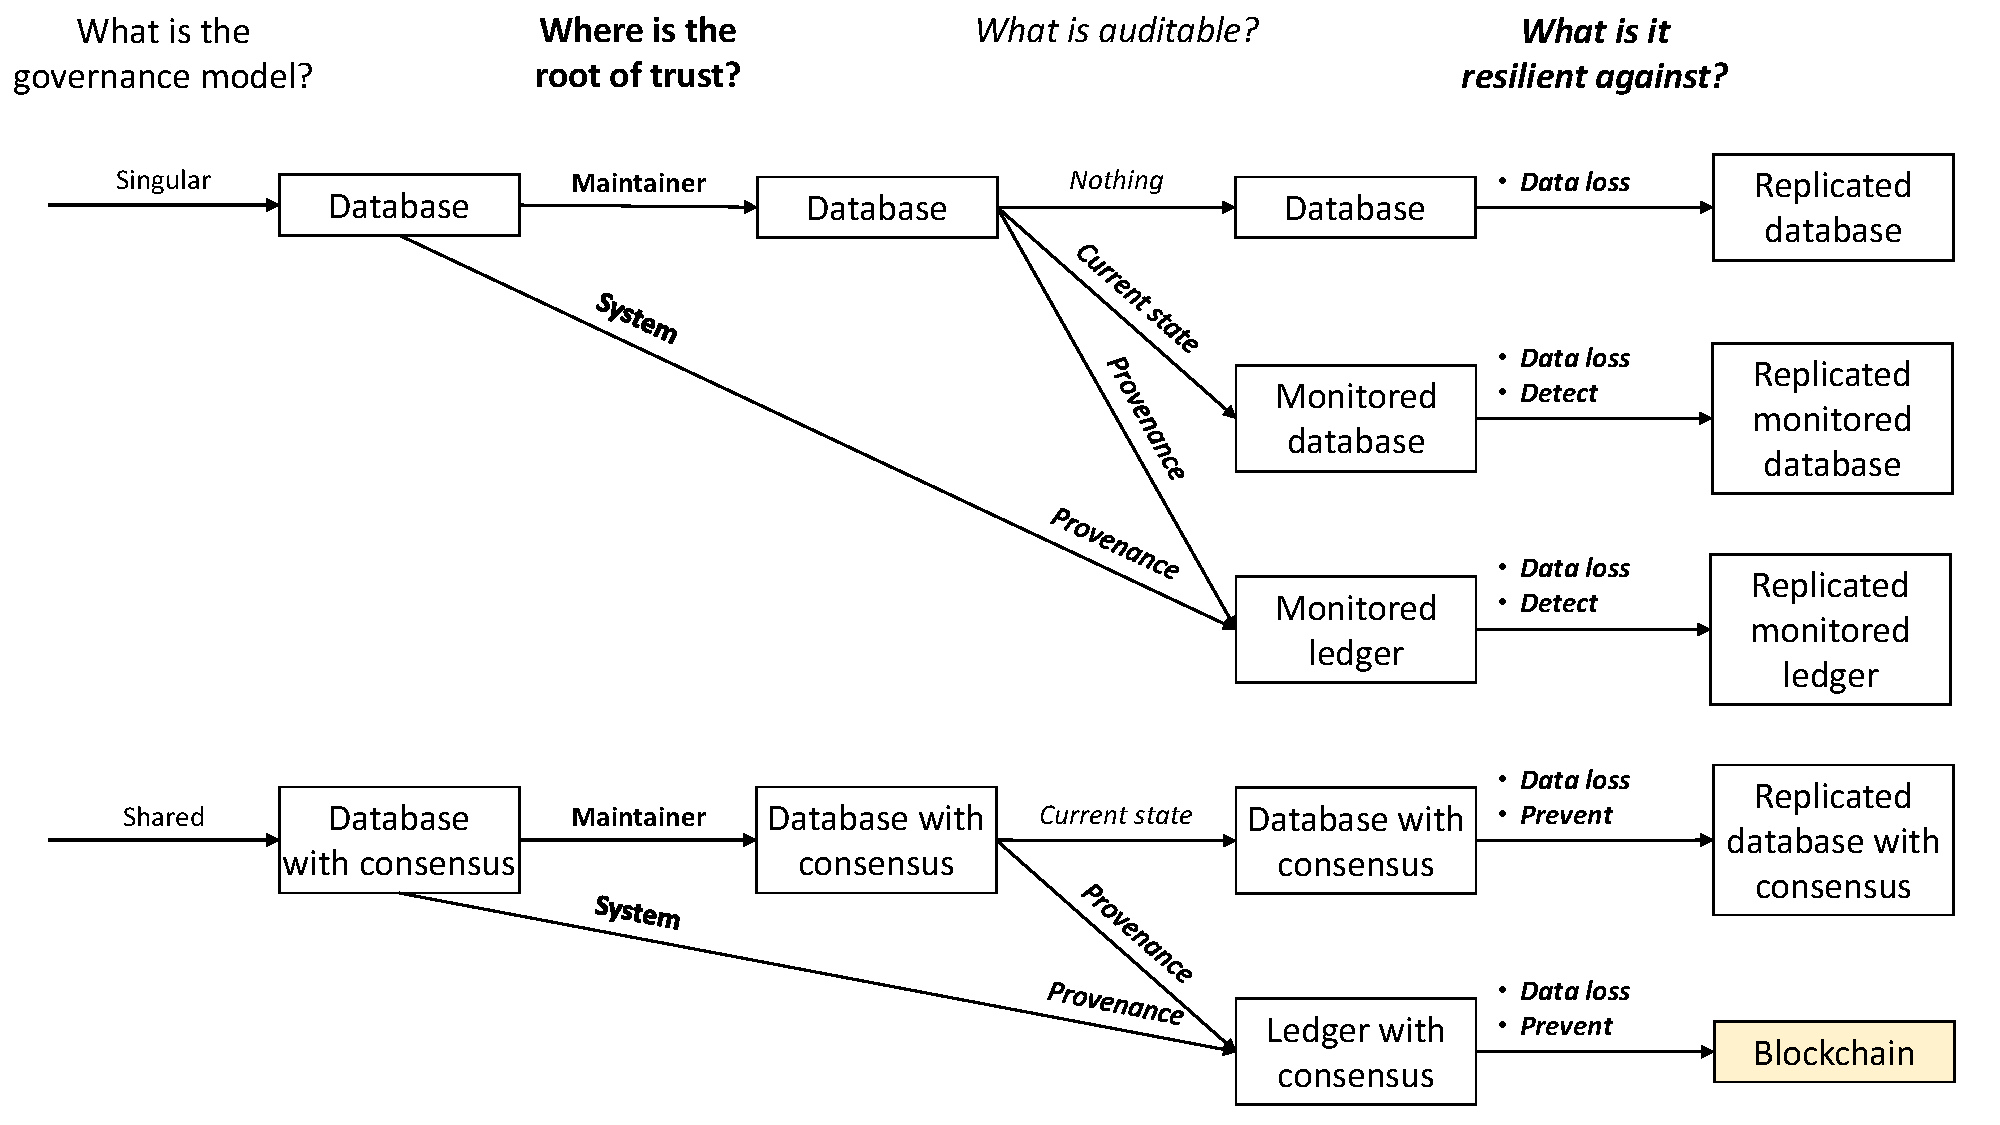
\includegraphics[width=\textwidth]{figures/BlockchainFlowchart}
	\caption{Comparing decentralized databases}
	\label{fig:blockchainFlowchart}
\end{figure*}

The first property in our taxonomy considers who has the authority to manage and update the database: \emph{what is the operation model?} In a singularly governed database (``Singular''), a single entity performs these tasks. Alternatively, the system can use a consensus protocol to allow for shared governance (``Shared'').

Next, we consider the security model by asking \emph{where is the root of trust?}
This refers to the entity or entities that must behave honestly in order for the system to be secure.
In typical database systems, trust is rooted in the maintainer (``Maintainer'')---for example, using AWS cloud storage requires that you trust Amazon.
Alternatively, trust can be rooted in the design of the system itself (``System''), though this is only possible if the system stores sufficient provenance for it to be audited to confirm that the system is functioning as intended.

The next question is \emph{what is auditable?}
In the worst case, nothing is auditable (``Nothing'').
Systems can use an authenticated data structure~\cite{tamassia2003authenticated} to ensure that their current state can be audited (``Current state'').
If the state also contains a history of the system (e.g., a ledger), then the use of an authenticated data structure allows for the provenance of the system to also be audited (``Provenance'').
In both cases, it is necessary that these databases be monitored to ensure that they never enter an invalid state, even temporarily.
In the case of shared operation, the operating entities act as monitors of the current sate during the consensus protocol.

Finally, we can classify systems by asking \emph{what is it resilient against?}
In particular, we considered with three resiliency properties---(1) is it resilient to accidental data loss (``Data loss''), (2) is it possible to detect that data has been malicious altered (``Detect''), (3) and is it possible to prevent malicious updates (``Prevent'').
Replication is a simple solution to prevent against accidental data loss, but by itself it fails to prevent malicious data loss as the malicious changes to the database will also be replicated.
In singular operation, external monitors can help detect malicious data changes, but can only do so after the data has been lost.
In shared operation, the monitors are the operators and malicious deletions and modifications will not be replicated, preventing them from effecting the overall system.
\section{Discussion}
In this section we discuss the remaining results from our grounded theory work.

\subsection{Normative properties}
\label{sec:normative}

\begin{figure}
	\centering
	\includegraphics[page=3,width=\columnwidth]{figures/grounded-theory-main}
	
	Arrows indicate that the destination depends on the source.
	\caption{Normative Properties for Blockchain Technology}
	\label{fig:normative-properties}
\end{figure}

Within the literature we analyzed, there were a set of properties that were not technical properties directly provided by Blockchain technology, but rather expressed desired properties for systems built using Blockchain technology (i.e., normative properties).
These properties are shown in Figure~\ref{fig:normative-properties}.

The majority of the normative properties focused around the notion of using Blockchain technology to allow for public participation.
While public participation is certainly possible with Blockchain technology, as there are many example of systems built using Blockchain technology that fail to achieve these properties.
For example, while Bitcoin initially had a low-cost to participate allowing easy-of-entry for miners and community ownership, that is no longer the case as any meaningful participation requires the purchase of a large amount of specialized hardware and the expenditure of a significant amount of electricity.

Similarly, the normative properties of low-bar for trust, disintermediation, no trusted third-parties, censorship resistance, and fast/cheap transaction all require extremely careful system design to achieve, and are not guaranteed by the use of Blockchain technology.
In practice, these properties are often difficult to guarantee for any system, and this is no different for Blockchain technology.
For example, Bitcoin ultimately requires trusted third parties (e.g., exchanges, retailers who accept Bitcoin) to allow the currency to be useful for real-world application.
Also, fast/cheap transactions usually only exist because Blockchain based systems are not yet regulated like non-Blockchain systems.

When reading documents from industry, normative and technical properties are often intermingled with each other.
The injection of ideology into a technical field causes confusion and suboptimal design choices, not to mention muddying discussion and preventing clarity.
Interestingly, in the concept graph generated by our methodology, the technical and normative properties were cleanly separated.
No capabilities have dependencies on normative properties, and removing them from the graph does not lessen the value of the graph as an exploration of technical concepts.
The fact that this separation occurred naturally provides evidence that grounded theory accomplished our research goals and was a good choice for addressing this corpus of data.

%In general, the normative properties dealt with idealogy-driven goals that could be accomplished using Blockchain technology.
%For example, several normative properties dealt with public participation, community ownership, censorship resistance, and transparency of Blockchain systems.
%Bitcoin demonstrates that Blockchain technology can be used to achieve these properties, but it is not the case that all Blockchain systems will accomplish these goals---for example, Ripple is a Blockchain system without public participation.

\subsection{Private Governance}
\label{sec:private-blockchain}
In our survey of the industrial literature, we encountered several proposals for Blockchain technology that used a centralized governance model where all miners are controlled by a single entity.
The most prominent example of a private governance system is IBM's HyperLedger Fabric.
Interestingly, the HyperLedger Fabric software project allows for consortium governance, but IBM's implementation has IBM run all of the miners.

Ultimately, we do not classify such systems as Blockchain technology.
First, these systems do not have shared governance, which we identify as the key component of Blockchain technology.
Second, the party governing the system still represents a single-point of failure.
While the miners within the operating organization might be run on a distributed infrastructure, there is still a high chance that a sufficient compromise in the operating organization would lead to a compromise in the Blockchain system.
Third, there is nothing that prevents the governing party from deleting or modifying data; even if such changes could be detected, the data itself is not replicated outside the organization and would be lost.
This is not to say that such systems lack value---such an evaluation is beyond the scope of this paper---but rather we believe that these types of systems are distinct from the more decentralized Blockchain technology.

\subsection{Lack of Privacy and Data Discoverability}
In the literature we found a common misconception that Blockchain technology inherently provided confidentiality for information stored within it.
In fact the opposite is true: all transactions are visible to all miners, and this is necessary for miners to validate transactions.
The global visibility was identified by some as a capability (i.e., data discoverability) that allowed a Blockchain to act as a data lake.
While there were some valid applications of Blockchain as a data lake, in most cases we found that proposed data lake applications did not need all of Blockchain technology's capabilities and that a simpler solution would have sufficed.
It may be possible to add confidentiality to Blockchain technology, but care must be taken to ensure that this confidentiality does not preclude miners' ability to validate and audit the system.
This remains an open research problem.

\subsection{Ideology, Hype, and Ulterior Motives}
Many proponents of Blockchain technology believe that it has the capability to massively disrupt how society operates, or at least to rapidly overtake legacy solutions in many significant industries. This belief is hyperbole, as though Blockchain technology has many valid uses, it has not, nor is it likely to achieve this Utopian vision. This ideology and hype causes problems: for example, frequent emotionally-charged schisms within Blockchain advocate and developer communities---especially those affiliated with Bitcoin. This turmoil prevents level-headed scientific discourse and wastes developer resources. It can also tangibly affect the stability of a Blockchain system by causing a fork in which two independent chains emerge to used and maintained by different groups, further dividing resources.

With that said, Blockchain's disruptive power has certainly been demonstrated in the financial sector, so it clearly has promise. Several factors have made this sector an attractive target for disruption, perhaps none more so than the opportunity for massive profit. This motive has had benefits for Blockchain, especially in accelerating the pace of technological development. However, it has also created perverse incentives to reinforce hype and ideology. Hype can attract investors and inflate valuations, and dogmatic ideology is a proven marketing and recruitment strategy for financial scammers. These problems inhibit the advancement of Blockchain technology.

\subsection{Reputation for illicit uses}
Due to the prominence of Bitcoin, many people are familiar with Blockchain first and foremost as the technology underlying the cryptocurrency and therefore the reputations of the two are intertwined. The fact that Bitcoin is designed to avoid banks and central authorities in general, combined with its well-known history of illicit uses, somewhat poisons the well for Blockchain as a whole. Along with the causes listed above (ideology, hype, and ulterior motives), this contributes to the difficulty of discussing and considering Blockchain technology with precision and objectivity. It may also have impeded or delayed its acceptance by organizations unwilling to associate themselves with the Bitcoin's poor reputation.
% !TEX root = ../main.tex
No content here.
% !TEX root = ../main.tex

\section{Related Works (Ben))}
Several prior authors have surveyed and systematized different aspects of the Blockchain landscape.
One of the most comprehensive works is from Bonneau et al., focusing on Bitcoin and other cryptocurrencies~\cite{BMC+15}. The authors seek to understand how Bitcoin has worked successfully and securely in practice for several years despite the lack of a rigorous model for its correctness and security. From a host of disparate sources, they distill a clear technical overview of how Bitcoin works. They then systematize the properties sufficient for system stability and analyze how they hold up under different assumptions about the incentives for miners. Finally, they evaluate and compare proposed changes to Bitcoin including tweaks to system parameters, alternative consensus protocols, and improvements to privacy and anonymity and conclude with a discussion of additional functionalities that Bitcoin could be extended to provide.  

Their approach differs from ours in several key ways, reflecting that our analyses have fundamentally different goals. They focus on a single application of Blockchain technology -- cryptocurrencies -- and survey technical sources in order to analyze how systems work and how design changes might affect functionality. By instead surveying sources that analyze Blockchain, we systematize the collective knowledge of the community to understand how Blockchain is being thought about and used by practitioners. This approach allows us to reason about how Blockchain may be useful in novel scenarios and to separate out normative beliefs from technical ones. 

Bano et al. focus on a particular technical component of Blockchain: the consensus process \cite{Bano17}. They systematize different protocols for consensus into three categories, identify shared characteristics and high-level design themes, and provide an evaluation framework to compare and contrast them. This paper serves an important purpose by connecting decades of "classical" research on consensus protocols to modern systems developed with Blockchain in mind. Our approach differs in scope and perspective, as we clarify not how Blockchain works technically but how analysts and users perceive it to work.

Another survey by Conti et al. focuses on security and privacy issues in Bitcoin\cite{Conti17}. The authors survey and tabulate known attacks against the Bitcoin network, miners, and clients as well as countermeasures and upgrade proposals that could improve privacy and anonymity in the system.  

Finally, Narayanan and Clark separated out the key technical ideas expressed in the design of Bitcoin and surveyed the academic lineage of each, repudiating the common belief that Bitcoin was a radical departure from existing research\cite{Narayanan17}. The authors discuss some aspects of how Bitcoin and Blockchain are understood by the general public, in particular identifying some key misconceptions that exist, but unlike in our work this is not their primary focus. Further, their survey covers academic literature while our goal of understanding how Blockchain is used and thought about by its users was best achieved by surveying analysis by industry and practitioners.
% !TEX root = ../main.tex

\section{Conclusion}
In this paper we answer three common questions regarding Blockchain technology: (1) what exactly is Blockchain technology, (2) what capabilities does it provide, and (3) what are good applications for Blockchain technology.
We accomplish this goal by analyzing a large corpus of data produced by industry using grounded theory.
This method was successfully able to help us separate Blockchain thought leadership provided by industry's best from the hype peddled by industry's worst.

Our results show that Blockchain technology provides several important properties that can be used in many interesting applications and use cases.  These include provenance, auditability, and access control and pseudonymity.
With these technical properties also comes significant overhead: shared governance and operation (i.e., consensus), as well as a fully replicated, auditable ledger.
As such, Blockchain technology is best suited for situations in which these properties are required and helpful for the given application or where the overhead can be minimized.

In short, we anticipate that Blockchain technology will be a tool used by industry going forward, supporting interesting and important research for both academic and industry security community members.

Even though it does not solve all the problems that its proponents claim it does, it is deserving of further research and application.

%====================================================================

%\bibliographystyle{abbrv}
%\bibliography{bib/bitcoin}
\bibliographystyle{IEEEtran}
\bibliography{bib/bitcoin}

%====================================================================

\appendix

\subsection{Relationship to other distributed systems}
\label{sec:distributed-comparison}
Blockchain technology fits within the broader family of distributed systems.
At the highest level, Blockchain technology is a type of decentralized database.
To help readers situate Blockchain technology within this greater ecosystem we have created a taxonomy and a flowchart based on that taxonomy (see Figure~\ref{fig:blockchainFlowchart}).

\begin{figure*}
	\centering
	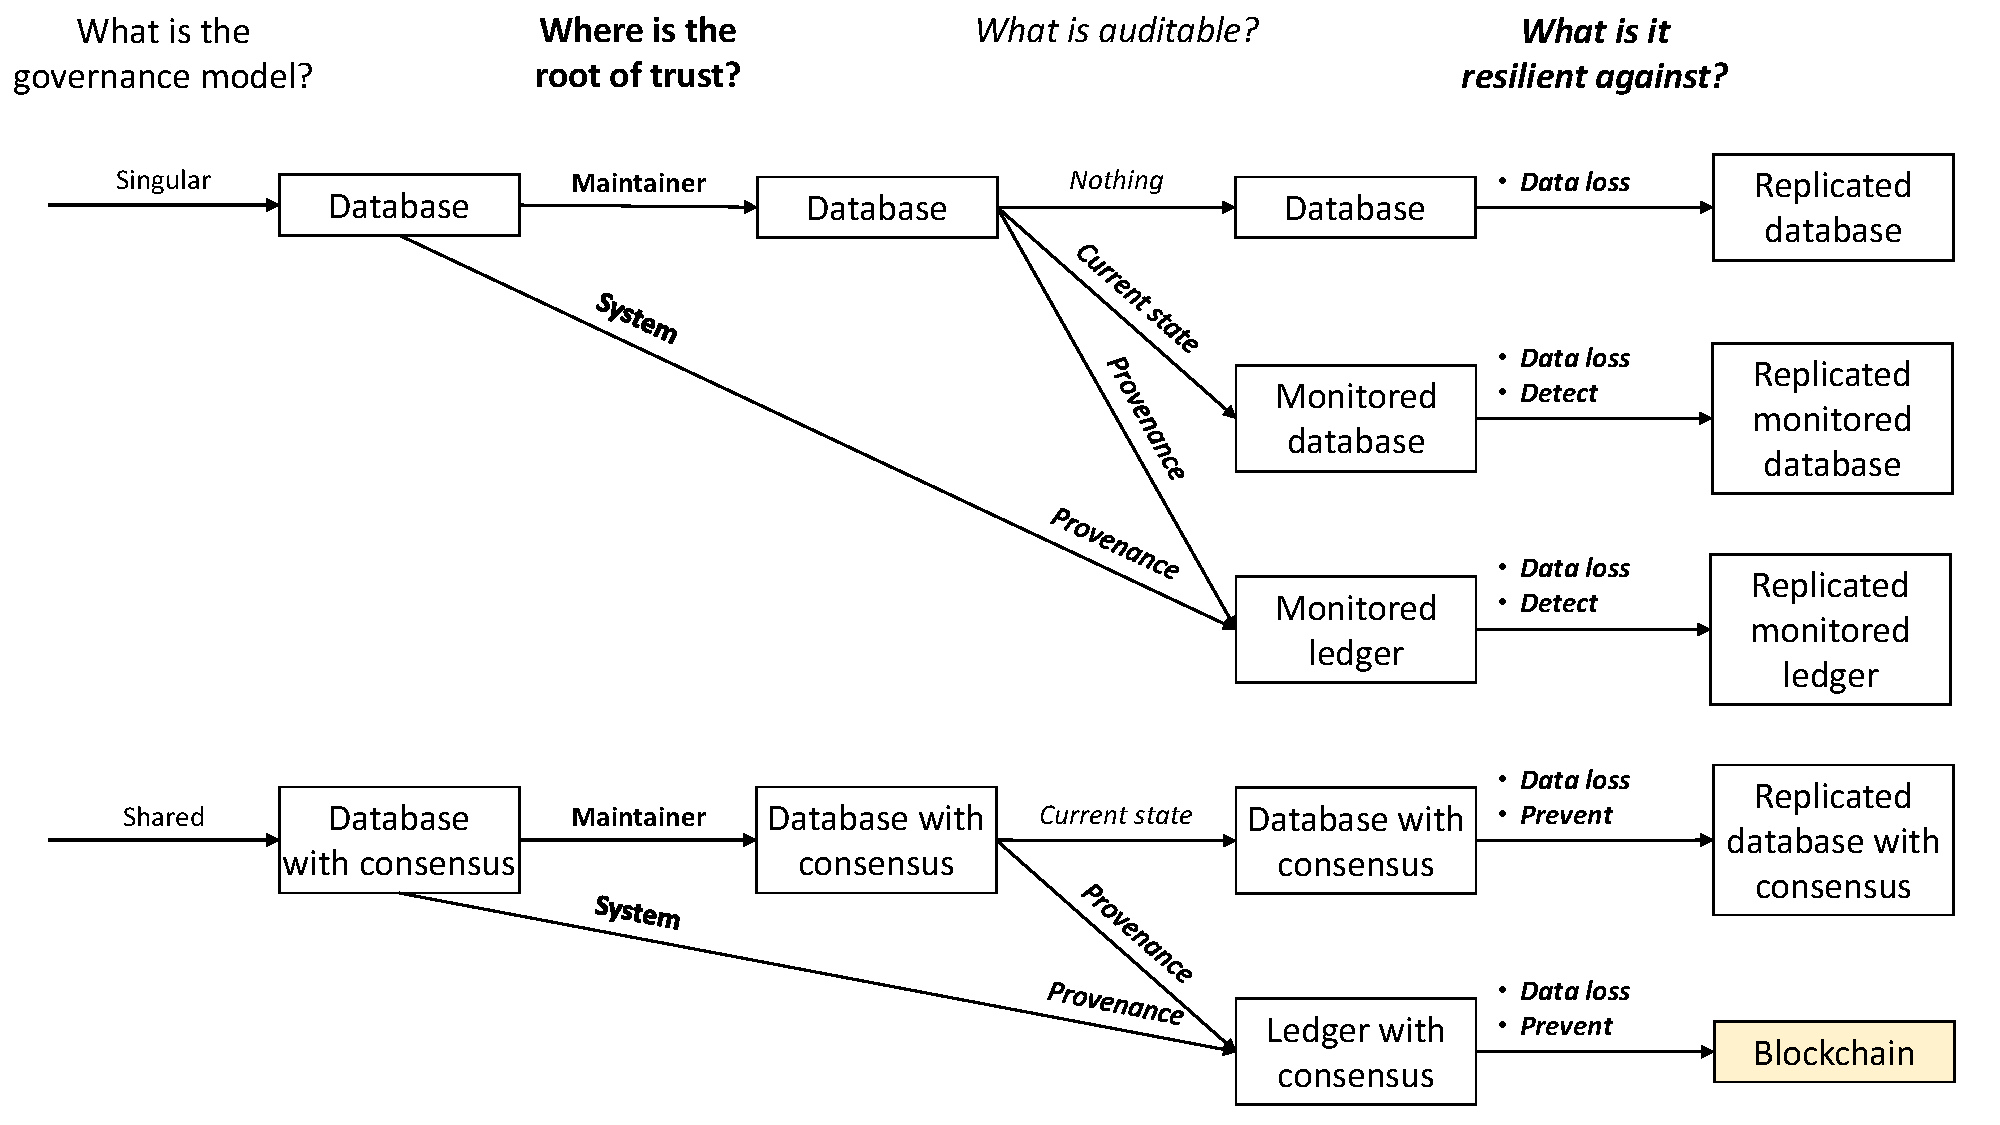
\includegraphics[width=.75\textwidth]{figures/BlockchainFlowchart}
	\caption{Comparing decentralized databases. Blockchain is highlighted in the bottom right corner.}
	\label{fig:blockchainFlowchart}
\end{figure*}

The first property in our taxonomy considers who has the authority to manage and update the database: \emph{what is the governance model?} In a centrally governed database (``Centralized''), a single entity performs these tasks. Alternatively, the system can use a consensus protocol to allow for decentralized governance (``Decentralized'').

Next, we consider the security model by asking \emph{where is the root of trust?}
This refers to the entity or entities that must behave honestly in order for the system to be secure.
In typical database systems, trust is rooted in the maintainer (``Maintainer'')---for example, using AWS cloud storage requires that you trust Amazon.
Alternatively, trust can be rooted in the design of the system itself (``System''), though this is only possible if the system stores sufficient provenance for it to be audited to confirm that the system is functioning as intended.

The next question is \emph{what is auditable?}
In the worst case, nothing is auditable (``Nothing'').
Systems can use an authenticated data structure~\cite{tamassia2003authenticated} to ensure that their current state can be audited (``Current state'').
If the state also contains a history of the system (e.g., a ledger), then the use of an authenticated data structure allows for the provenance of the system to also be audited (``Provenance'').
In both cases, it is necessary that these databases be monitored to ensure that they never enter an invalid state, even temporarily.
In the case of decentralized systems, the decentralized partners can act as monitors.

Finally, we can classify systems by asking \emph{what is it resilient against?}
In particular, we considered with three resiliency properties---(1) is it resilient to accidental data loss (``Data loss''), (2) is it possible to detect that data has been malicious altered (``Detect''), (3) and is it possible to prevent malicious updates (``Prevent'').
Systems with centralized governance are only able to detect malicious updates as the monitors can detect the attack but cannot prevent the malicious update from being replicated.
If we modify the system to allow monitors to play this role, they have become consensus partners and we now have a decentralized database.

\subsection{Survey of Academic Research on Challenges}
In this section, we report on a survey we conducted that looked at research from the academic community that attempts to address challenges related to and impeding the proper and secure use of Blockchain technology.

\subsubsection{Power consumption and centralization of mining}
To reduce the power consumption of Blockchain, there have been several proposals to turn to other consensus mechanisms that do not rely on proof of work.  The most popular of these proposals is proof of stake consensus, where parties' contribution to the consensus protocol is proportional to the total amount of stake they own in the system rather than the amount of work that they do.  This allows consensus to be achieved without relying on wasteful proofs of work.  Today's proof of stake protocols (e.g.~\cite{FC:BenGabMiz16,eprint:BenPasShi16,CRYPTO:KRDO17,SOSP:GHMVZ17}) vary significantly in their model, assumptions, and performance guarantees.  Other suggestions for avoiding proofs of work include proof of space~\cite{CRYPTO:DFKP15, eprint:PPKAFG15} where miners use storage instead of computation, and proof of elapsed time~\cite{SSS:CXSGLS17} where trusted hardware (i.e., Intel SGX) is used in place of proofs of work.  It is not clear at this point which solution will be best suited for different blockchain deployments.  

One possible solution~\cite{CCS:MKKS15} is to discourage mining pool formation by making it impossible to enforce cooperation between the members.

\subsubsection{Increasing transaction rates}
Another challenge to the scalability of Blockchain solutions, especially in the permissionless setting, is the increasing number of transactions.
Current systems often have rather long wait times before a transaction can be confirmed on the blockchain (e.g., Bitcoin can take several hours to confirm a transaction~\cite{BlockchainInfoTransactionConfTime}).  This makes blockchain-based solutions less than ideal when immediate transactions are needed, such as when purchasing physical goods.

A couple of different approaches have been proposed to deal with this issue.  First, a number of hybrid consensus algorithms (e.g.,~\cite{SOSP:GHMVZ17,OPODIS:AMNRS17,DISC:PasShi17,EC:PasShi18,NSDI:EGSR16}) aim to reduce transaction approval times through reducing or eliminating forks. Most of these work by using ``proof-of'' style protocols to elect a committee or a leader who then uses traditional byzantine fault-tolerant consensus to advance the blockchain.  A second approach for improving transaction rates, especially for financial transactions, is to make use of payment-channel networks. Such networks set up pairwise channels between parties to allow transactions on these channels to occur ``off-chain'', i.e., without being recorded on the blockchain; the blockchain is only used for conflict resolution.  Many different flavors of payment-channel networks achieving various properties have been proposed (e.g.~\cite{PooDry16, NDSS:HABSG17,CCS:KhaGer17,SYSTOR:LNEKPS18,CCS:MMKMR17,CCS:GreMie17}) and several such as the Lightning network~\cite{PooDry16} are in active development for financial transactions on top of Bitcoin.  

\subsubsection{Handling increased transaction volume}
Another scalability challenge for popular blockchain-based systems such as Bitcoin and Ethereum is the sheer volume of transactions that are being added to the blockchain.  As more and more third-party services start to use these blockchains to store and execute their transactions, these systems have to verify and store transactions for a variety of unrelated operations. This can cause the storage and verification work required of miners to become prohibitively expensive.

Proposed solutions for this problem include sharding (e.g.~\cite{CCS:LNZBGS16, FC:GenRenSir17}) to partition transactions based on the transaction type or service.
This allows different sets of miners to verify transactions for different services thus reducing the amount of verification work each miner must do.  Another more radical approach to deal with this challenge has been to move away from the ``chain'' view of blockchain.  Instead, several proposals (e.g., ~\cite{ePrint:SomLewZoh16,eprint:SomZoh18,IOTA}) propose to organize transactions into a directed-acyclic graph (DAG) where later transactions can vote on the validity of earlier transactions, allowing transactions to be approved before global consensus is achieved.

As the Bitcoin user base and transaction volume have grown, limitations on its scalability have been revealed. To some degree, these limitations are a result of Bitcoin's chosen parameters; for example, the 1MB cap on block size has periodically caused prohibitively high transaction fees and wait times. This limitation was mitigated by the Bitcoin Cash hard fork in 2017, which created 8MB blocks, but other scalability problems may not be so easily solvable by simple parameter tweaking, suggesting that they may be inherent limitations of public blockchain technology. We will discuss two limitations that stem from the proof-of-work consensus model that is typically used in public blockchains: emergent centralization of control and high rates of energy consumption.

Currently, almost 70\% of Bitcoin blocks are mined by the five largest pools \cite{BlockchainInfoPools}. Of course, these pools are disincentivized to damage trust in Bitcoin (and thus reduce its value and their profits) by abusing their power to censor transactions or violate rules in other ways. But this centralization undoubtedly runs counter to the normative property that Blockchain is decentralized and may violate security notions that depend on decentralization. This problem is caused in part by the hardware-optimized Bitcoin mining puzzle, for which alternatives are being explored, but whether or not this limitation can be overcome at scale is still an open question.

Bitcoin is also an illustrative example for another inefficiency of public blockchains at scale: the energy consumption of proof-of-work consensus. According to one estimate\cite{Digiconomist}, as of April 2018 the energy consumed by Bitcoin miners is equivalent to the power usage of almost 5.5 million US households, and all signs indicate that it will continue to grow. A similar problem is likely to arise in any scheme where proof-of-work is deployed. It may be surpassable if alternative consensus protocols such as proof-of-stake are used, but there are other problems to work out with such schemes (in particular, a worsening of the emergent centralization problem discussed above). 

\subsubsection{Smart contract correctness}
Three different directions have been proposed for improving the correctness and security of smart contracts:  Education and tools to help developers write smart contracts, tools for evaluating correctness and security of existing smart contracts, and formal modeling and formal verification of smart contracts. Along the education path, researchers organized a class on developing smart contracts cataloging common mistakes and misunderstandings~\cite{FC:DAKMS16}. Additionally, tools have been developed to simplify development of \emph{private} smart contracts~\cite{SP:KMSWP16}. For evaluation of existing smart contracts, multiple tools using symbolic execution~\cite{CCS:LCOSH16}, machine learning~\cite{arxiv:Huang18}, and static analysis~\cite{CCS:BDFGGK+16,NDSS:KGDS18} have been developed for detecting bugs and vulnerabilities. Finally, some efforts to support development of formally verified smart contracts is underway; for example, the Ethereum Virtual Machine (EVM) has been fully defined for interactive theorem provers~\cite{Hirai17}, which are essential tools for building formally verified software of any kind. Magazzeni et al.~\cite{Magazzeni17} have laid out a research agenda identifying further groundwork that must be conducted to support formal verification of smart contracts.

\subsubsection{Dispute resolution and rollback of mistakes}
Despite best efforts to eliminate mistakes in smart contract and transactions, a payment or asset transfer system must be able to reverse fraudulent or errant transactions. The immutability property of Blockchain means that transactions cannot be stricken from the ledger after consensus has been reached, so alternative means of dispute resolution must be explored. A new transaction reversing the effects of the disputed transaction could be added to the ledger, but decentralized governance makes arbitrating such a dispute difficult as there is no individual arbiter with the authority to determine which party is in the right when a dispute occurs.  Additionally, dispute resolution must be handled carefully to avoid introducing new vulnerabilities.  For example, several attacks were demonstrated against the Bitcoin refund mechanism~\cite{FC:MccShaHao16} necessitating further research to design secure refunds in Bitcoin~\cite{arxiv:AviSafSha18}.

\subsubsection{Non-auditability of off-chain oracles}
Smart contracts sometimes leverage off-chain oracles: online services that provide information in response to a request. For example, gambling contracts may determine which address to pay winnings to based on the result of some oracle request (e.g., sports scores, stock prices, weather forecasts, or other global events). If contract logic branches based on the response from an off-chain oracle, that contract is no longer verifiable after the fact because auditors cannot confirm that the response received from the oracle at audit time is the same response received when the contract was executed. There are legitimate reasons why an oracle response might change with time, so this is really an inherent limitation of Blockchain technology: smart contracts cannot "see" external events.

One system tackling this problem is Town Crier~\cite{Zhang16}. It uses a trusted hardware back end (Intel SGX) to serve as an authenticated off-chain oracle for Ethereum smart contracts. This allows an auditor to later verify the oracle's response at the time at which the contract was executed. This solution sidesteps the limitation of oracle non-auditability by moving trust to a centralized location (the hardware platform providing authenticity), but it does not diffuse trust in the way our analysis reveals that Blockchain technology is expected to.

\subsection{Key Management}
Another major challenge of blockchain is that it requires users to store, manage, and secure cryptographic keys both to certify their own transactions and to verify transactions of others.  However, the challenges of maintaining and protecting such key repositories are well documented (see, e.g.~\cite{uss:WhiTyg99}).  A survey by Eskandari et al.~\cite{arxiv:ECBS18} outlines the challenges as well as potential solutions for managing keys for Bitcoin.  They discuss solutions such as password-protected and password-derived keys as well as offline and air-gapped storage of the keys.  But, as the authors state all of these solutions have their drawbacks.

Some recent work has also looked into cryptographic solutions to protect users' keys.  Techniques based on secure multi-party computation (MPC)~\cite{CCS:LinNof18,C:Lindell17} allow transactions to be signed without any party ever having access to the secret key.  Alternatively, the classic technique of threshold signatures (e.g.~\cite{PKC:Boldyreva03,EC:GJKR96,EC:Shoup00a}) allow users to split their keys into many pieces such that a large number of them must be compromised in order to ``steal'' a user's key.  However, much work remains to secure all the cryptographic keys inherent in real-world blockchain deployments.


\subsection{Technical Properties Full Diagram}

\begin{center}
	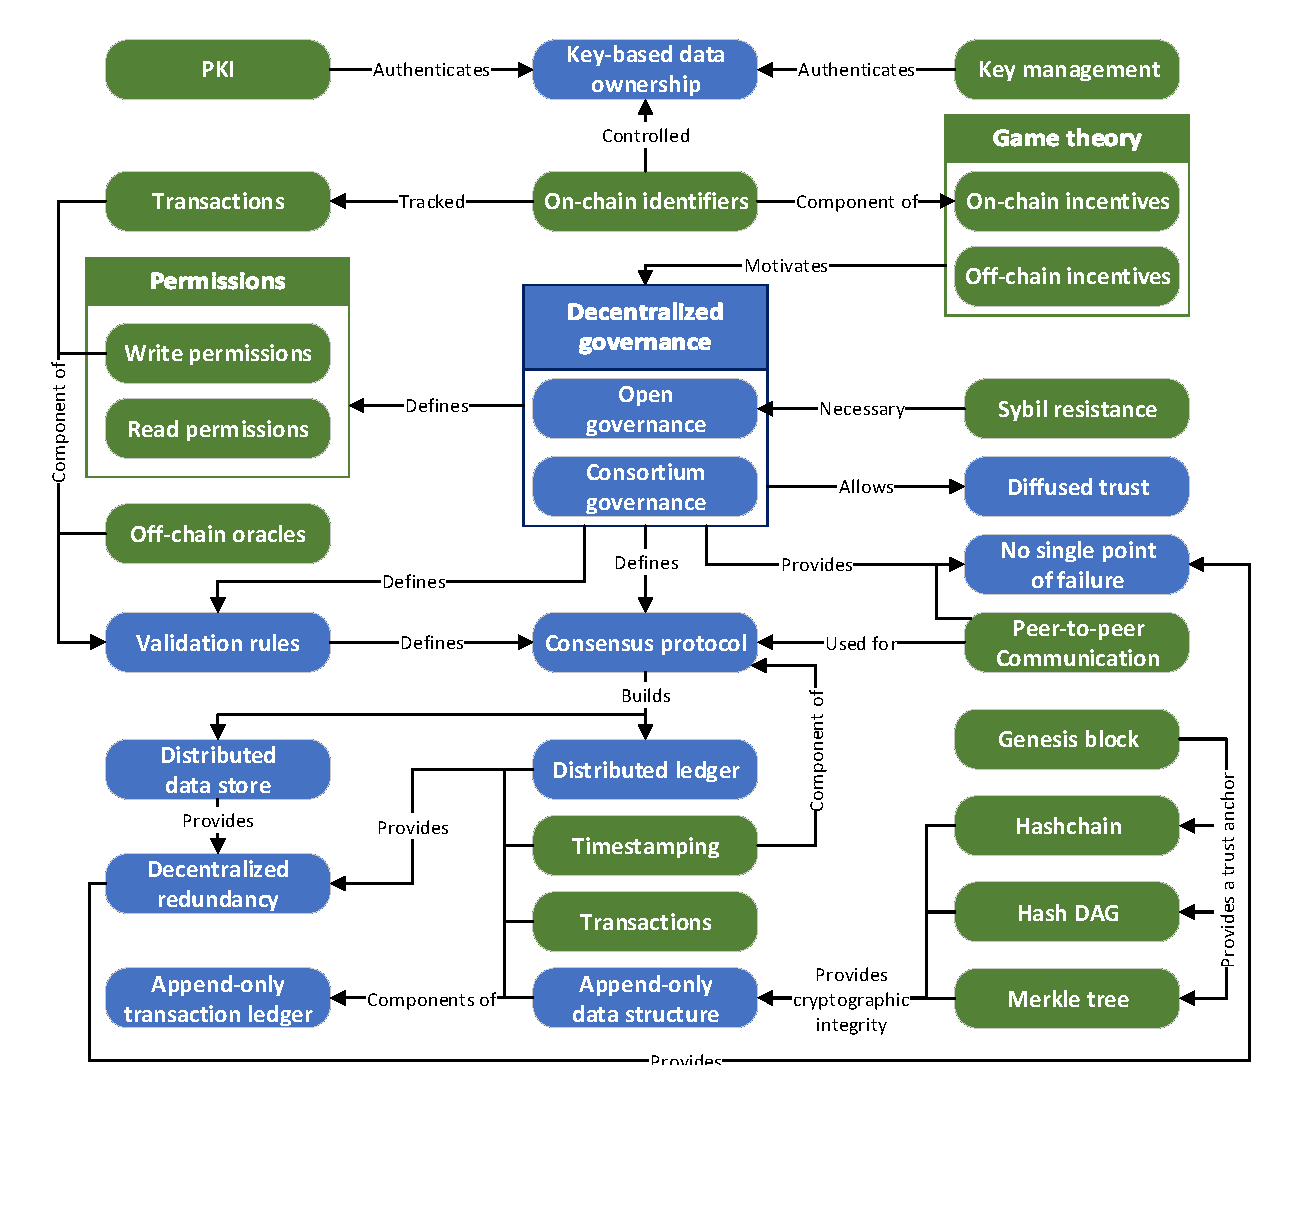
\includegraphics[page=1,width=\columnwidth]{figures/grounded-theory-main}
	\captionof{figure}{Technical Properties for Blockchain Technology With Supporting Technical Primitives}
	\label{fig:technical-properties-full}
\end{center}

%\begin{figure}
%	\centering
%	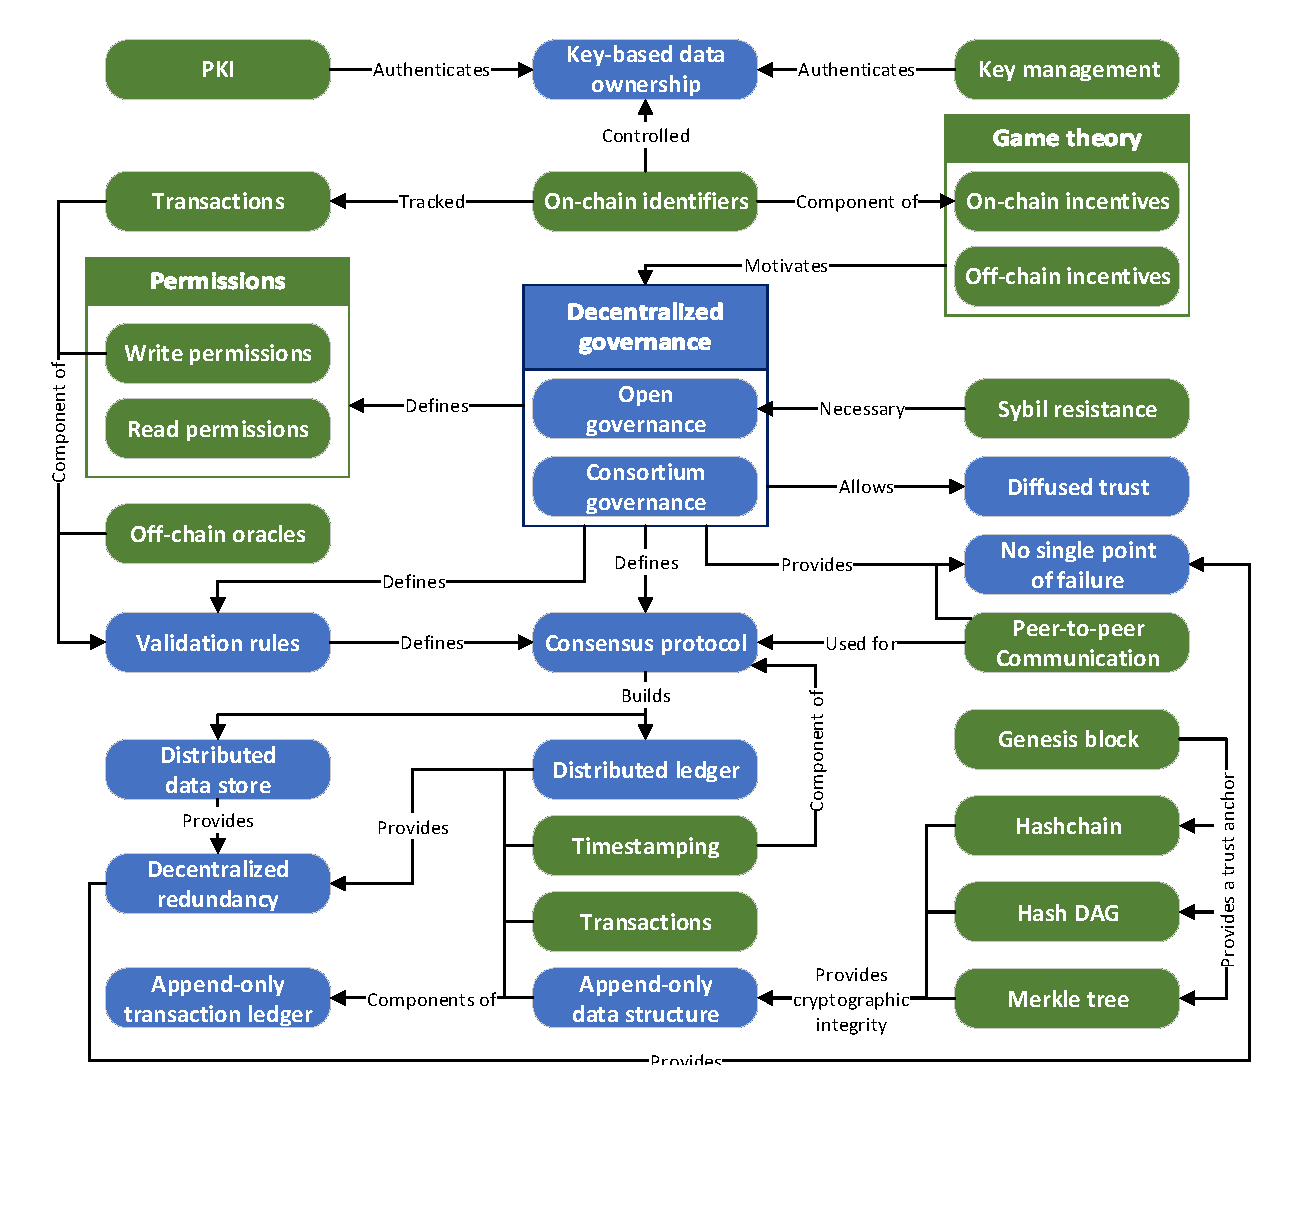
\includegraphics[page=1,width=\columnwidth]{figures/grounded-theory-main}
%	
%	Technical properties are in blue and technical primitives are in green.
%	\caption{Technical Properties for Blockchain Technology With Supporting Technical Primitives}
%	\label{fig:technical-properties-full}
%\end{figure}

%====================================================================

\end{document}


